 % arara: pdflatex: { synctex: yes }
% arara: makeindex: { style: ctuthesis }
% arara: bibtex

% The class takes all the key=value arguments that \ctusetup does,
% and a couple more: draft and oneside
\documentclass[twoside]{ctuthesis}
\usepackage{graphicx}
\usepackage{adjustbox}
\usepackage{makecell}
\usepackage[colorinlistoftodos]{todonotes}
\usepackage[sortlocale=cs_CZ, sorting=debug, style=iso-numeric, maxnames=2]{biblatex}
\usepackage{array,etoolbox}
\usepackage{xcolor}
\usepackage{caption}
\usepackage{subcaption}
\usepackage{enumitem}
\usepackage{indentfirst}
\usepackage{multirow}
\usepackage{multicol}
\usepackage{chngpage}
\usepackage{rotating}
\usepackage[acronym,nomain,nonumberlist]{glossaries}
\makenoidxglossaries

\renewcommand{\glossarysection}[2][]{}

\newacronym{ui}{UI}{Uživatelské rozhraní}
\newacronym{dpp}{DPP}{Dohoda o~provedení práce}
\newacronym{dpc}{DPČ}{Dohoda o~pracovní činnosti}
\newacronym{mvc}{MVC}{Model-View-Controller}
\newacronym{mvvm}{MVVM}{Model-View-ViewModel}
\newacronym{uc}{UC}{Use Case (případ užití)}
\newacronym{dao}{DAO}{Data Access Object}
\newacronym{rest}{REST}{Representational state transfer}
\newacronym{api}{API}{Application Programming Interface}


\newacronym{json}{JSON}{JavaScript Object Notation}
\newacronym{crud}{CRUD}{Create, Read, Update, Delete}
\newacronym{html}{HTML}{Hypertext Markup Language}
\newacronym{xml}{XML}{Extensible Markup Language}
\newacronym{bco}{BCO}{Bee Colony Optimization}
\newacronym{abc}{ABC}{Artificial Bee Colony}
\newacronym{sql}{SQL}{Structured Query Language}
\newacronym{orm}{ORM}{Object Relation Mapping}
\newacronym{id}{ID}{Identifikátor}

\newacronym{dsl}{DSL}{Domain-specific language}
\newacronym{http}{HTTP}{Hypertext Transfer Protocol}
\newacronym{url}{URL}{Uniform Resource Locator}
\newacronym{mvp}{MVP}{Model-View-Presenter}
\newacronym{ide}{IDE}{Integrated Development Environment}

\newacronym{rpc}{RPC}{Remote Procedure Call}
\usepackage{listings}

\graphicspath{{img/}}

\preto\tabular{\setcounter{magicrownumbers}{0}}
\newcounter{magicrownumbers}
\newcommand\rownumber{\stepcounter{magicrownumbers}\arabic{magicrownumbers}}

\renewcommand*{\finalnamedelim}{ a }
\ctusetup{
	mainlanguage = czech,
	otherlanguages = {slovak, english},
	title-czech = {Mobilní aplikace pro plánování lidských zdrojů},
	title-english = {Mobile App for Human Resource Planning},
	doctype = S,
	faculty = F3,
	department-czech = {Katedra počítačů},
	department-english = {Department of Computer Science},
	author = {Martina Kopecká},
	supervisor = {Ing. Jiří Šebek},
	supervisor-address = {TODO},
	fieldofstudy-english = {Software Engineering -- TODO, co je ENG nazev},
	fieldofstudy-czech = {Softwarové inženýrství a technologie},
	keywords-czech = {slovo, klíč},
	keywords-english = {word, key},
	day = 4,
	month = 1,
	year = 2021,
	pkg-listings = true,
}


\definecolor{codegreen}{rgb}{0,0.6,0}
\definecolor{codegray}{rgb}{0.5,0.5,0.5}
\definecolor{codepurple}{rgb}{0.58,0,0.82}
\definecolor{backcolour}{rgb}{0.88,0.96,0.98}
\definecolor{NavyBlue}{RGB}{255,137,0}
\definecolor{OrangeRed}{RGB}{225,118,242}
\definecolor{BurntOrange}{rgb}{0.88,0.96,0.98}
\definecolor{ForestGreen}{RGB}{18,91,10}

\lstdefinelanguage{Kotlin}{
  comment=[l]{//},
  commentstyle={\color{gray}\ttfamily},
  emph={delegate, filter, first, firstOrNull, forEach, lazy, map, mapNotNull, println, return@},
  emphstyle={\color{OrangeRed}},
  identifierstyle=\color{black},
  keywords={abstract, actual, as, as?, break, by, class, companion, continue, do, dynamic, else, enum, expect, false, final, for, fun, if, import, in, interface, internal, is, null, object, override, package, private, public, return, sealed, set, super, suspend, this, throw, true, try, typealias, val, var, vararg, when, where, while},
  keywordstyle={\color{NavyBlue}\bfseries},
  morecomment=[s]{/*}{*/},
  morestring=[b]",
  morestring=[s]{"""*}{*"""},
  ndkeywords={@Deprecated, @JvmField, @JvmName, @JvmOverloads, @JvmStatic, @JvmSynthetic, Array, Byte, Double, Float, Int, Integer, Iterable, Long, Runnable, Short, String, T},
  ndkeywordstyle={\color{ctublue}\bfseries},
  sensitive=true,
  stringstyle={\color{ForestGreen}\ttfamily},
}

\ctuprocess

\addto\ctucaptionsczech{%
	\def\supervisorname{Vedoucí}%
	\def\subfieldofstudyname{Studijní program}%
}

\ctutemplateset{maketitle twocolumn default}{
	\begin{twocolumnfrontmatterpage}
		\ctutemplate{twocolumn.thanks}
		\ctutemplate{twocolumn.declaration}
		\ctutemplate{twocolumn.abstract.in.titlelanguage}
		\ctutemplate{twocolumn.abstract.in.secondlanguage}
		\ctutemplate{twocolumn.tableofcontents}
		\ctutemplate{twocolumn.listoffigures}
	\end{twocolumnfrontmatterpage}
}

\lstdefinestyle{mystyle}{
    backgroundcolor=\color{backcolour},
    commentstyle=\color{codegreen},
    keywordstyle=\color{magenta},
    numberstyle=\tiny\color{codegray},
    stringstyle=\color{codepurple},
    basicstyle=\ttfamily\footnotesize,
    breakatwhitespace=false,
    breaklines=true,
    captionpos=b,
    keepspaces=true,
    numbers=left,
    numbersep=5pt,
    showspaces=false,
    showstringspaces=false,
    showtabs=false,
    tabsize=2,
		extendedchars=false,
    inputencoding=utf8,
		texcl=true,
		literate={é}{{\'e}}1
           {č}{{\v{c}}}1
           {ľ}{{\v{l}}}1
           {ť}{{\v{t}}}1
           {ý}{{\'y}}1
           {ě}{{\v{e}}}1
           {ř}{{\v{r}}}1
           {š}{{\v{s}}}1
           {ž}{{\v{z}}}1
           {á}{{\'a}}1
           {í}{{\'i}}1
           {ó}{{\'o}}1
           {ň}{{\v{n}}}1
           {ď}{{\v{d}}}1
           {ú}{{\'u}}1
           {ů}{{\r{u}}}1
           {ĺ}{{\v{l}}}1
					 {Ž}{{\v{Z}}}1
					 {Č}{{\v{C}}}1
					 {Ř}{{\v{R}}}1
					 {Í}{{\'{I}}}1
}

\renewcommand\lstlistingname{Výpis kódu}

\setlength{\parskip}{0.5em}
% \setlength{\parskip}{5ex plus 0.2ex minus 0.2ex}

% Abstract in Czech
% \begin{abstract-czech}
% Český abstrakt
% \end{abstract-czech}

% Abstract in English
% \begin{abstract-english}
% English abstract
% \end{abstract-english}

% Acknowledgements / Podekovani
\begin{thanks}
Děkuji Ing. Jiřímu Šebkovi za cenné rady k~vypracování této práce.
\end{thanks}

% Declaration / Prohlaseni
\begin{declaration}
Prohlašuji, že jsem předloženou práci vypracovala samostatně s~použitím uvedené literatury.

V Praze, \ctufield{day}.~\monthinlanguage{title}~\ctufield{year}
\end{declaration}

\DeclareLabeldate[article]{
  \field{date}
  \field{year}
  \field{eventdate}
  \field{origdate}
  \field{urldate}
}

\addbibresource{bibliography.bib}
\lstset{style=mystyle}

\begin{document}

\maketitle

%
\chapter{Úvod}

V~dnešní době neustále stoupá podíl uživatelů, kteří na některé běžné činnosti na síti (vyhledávání informací, chatování, internetové bankovnictví, čtení a psaní e-mailů,~\ldots) nezapínají počítač, a namísto toho používají svůj chytrý telefon. Téměř vše, co aktuálně potřebují, tak mají rychle dostupné na zařízení, které mají neustále s~sebou.

Vzhledem k~rozvoji mobilní platformy a trendu růstu její oblíbenosti tedy neexistuje důvod, proč by uživatelé (v~tomto případě tedy zaměstnanci, kteří mají nepravidelný pracovní rozvrh -- ať už se jedná o~pracovníky v~restauracích, obchodech, továrnách nebo např.~o~zdravotníky) nemohli mít na svém zařízení snadno dostupný i~rozpis svých směn, namísto toho, aby ho hledali na nástěnce, v~tabulkovém editoru nebo kdekoli jinde.

Právě proto je cílem této práce analyzovat, navrhnout a im\-ple\-men\-to\-vat uživatelsky přívětivý způsob, jakým by šlo aktuální rozvrh směn do chytrých telefonů dostat, a usnadnit (a snad i zpříjemnit) tak život nejen zaměstnancům, ale i~vedoucím pracovníkům.
% TODO


\chapter{Analýza problematiky}
Následující kapitola bude věnována analýze problematiky plánování lidských zdrojů, a to jednak z~hlediska terminologie, jednak z~hlediska manažerského a právního (důraz je zde kladen především na pracovní dobu a typy pracovněprávních vztahů v~české legislativě a rozdíly mezi nimi).

\section{Definice a terminologie}

Řízení lidských zdrojů (angl. human resource management\footnote{Také se užívá pojem people management, neboť pojem human resources může mít negativní konotace a~značit, že lidé jsou stejným zdrojem ve výrobě jako cokoli jiného. \cite[s.~1]{armstrong2014} Samotné spojení human resources se používá ve spojitosti s~personálním oddělením v~rámci organizace. }) je definováno jako komplexní přístup k~zaměstnávání a rozvoji osob. Pojem v~sobě obecně zahrnuje všechny aspekty toho, jak jsou osoby zaměstnány a řízeny v~rámci organizace. \cite[s.~1]{armstrong2014}

Dalším termínem užívaným v~literatuře je pracovní síla (angl. workforce nebo manpower), resp. její plánování, jedná se o základní proces řízení lidských zdrojů, který je utvářen strategií organizace a jeho cílem je zajistit, aby správný počet lidí se správnými schopnostmi, na správném místě, ve správném čase, za správnou cenu a~ve správném pracovněprávním poměru pomáhal organizaci dosáhnout jejích cílů. Mezi kroky tohoto procesu dle \cite{cipd2020workforce} patří:
\begin{itemize}
	\item analýza aktuální personální situace;
	\item stanovení budoucích potřeb;
	\item identifikace současných nedostatků vzhledem k~plánu do budoucna;
	\item podnikání akcí k~odstranění nedostatků;
	\item sledování a vyhodnocení dopadů akcí.
\end{itemize}
% \todo{Kde si v~tom stojí rozvrhování?}

\section{Rozhodující faktory při plánování}
% PESTLE analyza

\subsection{Pracovní síly}
V rámci organizace mohou existovat rozdíly mezi jednotlivými pracovníky. Jen část zaměstnanců tak bude pracovat na plný úvazek, jiní mohou pracovat méně hodin, například pouze v nejvytíženějších dnech \cite{lin2015}. V případě těchto zaměstnanců, kteří pracují méně hodin (a ne vždy pravidelně), je třeba zohlednit různé typy pracovněprávních vztahů, čemuž bude věnován prostor dále v~podkapitole \ref{section:legislativa}. Individualitu zaměstnanců je třeba zohlednit i z~důvodu rozdílů mezi jejich schopnostmi.
% Dalším hlediskem, které je vhodné brát v~úvahu, je i spokojenost zaměstnanců, jejich časové možnosti a preference.

\subsection{Směny}
\label{sub:smeny}
Jednotlivé organizace se od sebe mohou lišit způsobem, jakým vypisují směny. Existují tak podniky, kde je rozvrh práce pravidelný a stejný pro všechny zaměstnance, ale i ty, kde je provoz dvou- nebo i třísměnný, rozvrh směn je sestavován cyklicky a začátek směn daného zaměstnance se v~jed\-not\-li\-vý\-ch dnech liší (tedy např. jeden den má směnu ranní a další den noční). Mezi organizace s~cyklicky sestavovaným rozvhem se řadí nejčastěji provozy, které jsou vz~provozu 7~dní v~týdnu, například nemocnice, vězení, policie nebo také restaurace a pobočky řetězců rychlého občerstvení \cite{bechtold1981work}.

Nepravidelný rozvrh směn přitom může mít pro zaměstnance nežádoucí zdravotní účinky, např.~\cite{flo2013shift} uvádí, že zaměstnanci ve vícesměnném provozu trpí nespavostí více než zbytek populace, a to především v~případě, že je mezi směnami kratší než 11hodinová přestávka.

% \subsection{Úkoly}
% TODO -- může to být sekvence činností při směně nebo fakt, že teď pracuje organizace na něčem?

% V~případě, že zaměstnanci jsou při práci vystaveni zdravotním rizikům, je vhodné během směny rozdělit úkoly tak, aby riziko bylo minimalizováno. \cite{wongwien2013ergonomic}

% Provozní úkoly (angl. operational tasks) jsou běžné činnosti, které musí během dne zaměstnanci vykonat \cite{lin2015}. Při jejich plnění se přitom nevytváří nový produkt, ale udržuje se chod organizace (např. se jedná o~administrativní úkoly). Lze je rozdělit na prioritní, plánované a neplánované \cite{miwa2010}.

\subsection{Předpověď poptávky po personálu}
\label{sub:demand}
Obecně řečeno musí zaměstnanci plnit úkoly podle toho, jaké události nastanou. Modelováním poptávky se rozumí proces, jehož výstupem je předpověď přibližného počtu zaměstnanců a jejich očekávaných kompetencí \cite[s.~219]{armstrong2014}, a to na základě očekávaných událostí \cite{ernst2004staff}.

Například prodejce hraček tedy na základě historických dat ví, že nejvíce zákazníků přichází před Vánoci a předpokládá, že tomu tak bude i v~následujícím roce. Na tuto událost bude reagovat tím, že se rozhodne rozšířit otevírací dobu. To celkově zvýší poptávku po personálu v~daném období.

\subsection{Cena}
Dalším důležitým faktorem při plánování pracovních sil je celková cena lidské práce a otázka její optimalizace při naplnění poptávky.


\section{Legislativní podmínky}
\label{section:legislativa}
Hlavním právním předpisem, který se upravuje problematiku pracovních sil, je v~českém prostředí zákoník práce, který upravuje vztahy vznikající při výkonu závislé práce mezi zaměstnanci a~zaměstnavateli, tedy pracovněprávní vztahy \cite{zakonik06-262}.

Zaměstnavatel je dle §~38 zákoníku práce povinen přidělovat zaměstnanci práci podle pracovní smlouvy. Zaměstnanec je pak povinen podle pokynů zaměstnavatele konat osobně práci v~rozvržené týdenní pracovní době.

\subsection{Pracovní doba}
Pracovní dobou se rozumí doba, v~níž je zaměstnanec povinen vykonávat práci pro zaměstnavatele nebo je k tomu na pracovišti připraven. Doba odpočinku není součástí pracovní doby. (§ 78 zákoníku práce)

Stanovená týdenní pracovní doba činí dle §~79 zákoníku práce 40~hodin (mimo výjimky). Pracovní dobu rozvrhuje zaměstnavatel, který určuje začátek a konec směn, a to zpravidla do pětidenního pracovního týdne (§ 81). Délka směny nesmí přesáhnout 12~hodin. U nezletilých zaměstnanců pak nesmí délka směny v~jednotlivém dni překročit 8~hodin a v~jednom týdnu 40~hodin.

\subsection{Rozvrh pracovní doby}
Zaměstnavatel je dle §~84 zákoníku práce povinen vypracovat rozvrh týdenní pracovní doby a seznámit s~ním nebo jeho změnou zaměstnance nejpozději 2~týdny předem (mimo výjimky stanovené zákonem nebo v~případě existence jiné dohody mezi zaměstnancem a zaměstnavatelem). Tento rozvrh musí být v~písemné formě. Pracovní dobu je podle §~90 třeba rozvrhovat s ohledem na nepřetržitý odpočinek mezi koncem jedné směny a začátkem následující (pro zletilé zaměstnance alespoň 11 hodin, pro nezletilé zaměstnance alespoň 12 hodin, v~zákonem stanovených výjimkách lze za určitých podmínek odpočinek zkrátit).

\subsection{Směna, směnný provoz}
Směnou se dle §~78, písm. c) zákoníku práce rozumí část týdenní pracovní doby bez práce přesčas, kterou je zaměstnanec povinen na základě předem stanoveného rozvrhu pracovních směn odpracovat.

\subsection{Pracovní poměr}
Pracovní poměr mezi zaměstnancem a zaměstnavatelem se podle §~33, odst.~1 zákoníku práce zakládá pracovní smlouvou. Zaměstnavatel má zajišťovat plnění svých úkolů především zaměstnanci v pracovním poměru (§~74, odst.~1).

\subsection{Zkrácený úvazek}
Podle §~80 zákoníku práce může být mezi zaměstnancem a~zaměstnavatelem sjednána kratší pracovní doba.

\subsection{Dohody o pracích konaných mimo pracovní poměr}
§~77 zákoníku práce stanovuje, že na práci konanou na základě dohod o pracích konaných mimo pracovní poměr se vztahuje úprava pro výkon práce v~pracovním poměru, a to mimo výjimky uvedené v odst.~2 tohoto paragrafu (např. pracovní dobu a~dobu odpočinku nebo dovolenou). Podle §~74 přitom zaměstavatel není zaměstnancům na dohody povinen rozvrhnout pracovní dobu.

\subsubsection{Dohoda o provedení práce}
Podle §~75 zákoníku práce se dohoda o provedení práce uzavírá nejvýše na 300~hodin v~kalendářním roce (doba se u jednoho zaměstnavatele sčítá v~případě, že je dohod uzavřeno více).

\subsubsection{Dohoda o pracovní činnosti}
Podle §~76 zákoníku práce není na základě dohody o pracovní činnosti možné vykonávat práci v~rozsahu překračujícím v~průměru polovinu stanovené týdenní pracovní doby. Toto se posuzuje za celou dobu, po niž je uzavřena, nejdéle však za 52 týdnů. Musí být sjednán rozsah pracovní doby a doba, na niž se sjednává.


\chapter{Analýza systému}

Cílem této práce je navrhnout mobilní aplikaci pro plánování lidských zdrojů, obzvláště rozvrhování směn. Bude se tak jednat o aplikaci, která bude sloužit pro zjednodušení interních procesů v~rámci nějaké firmy, půjde o~minimalistický informační systém pro zaměstnance a zaměstnavatele. Pro účely identifikace požadavků bude v~této kapitole vytvořen předpoklad o~cílové skupině organizací, které by mohly tento software nasadit, jaká je jejich současná situace a co by jim mělo toto softwarové řešení poskytnout. Rovněž budou z~uživatelského pohledu popsána již existující softwarová řešení, která jsou pro dané situace určena.

\section{Cílová skupina}
Pro účely stanovení požadavků byl vytvořen předpoklad o~cílové skupině pro tento systém: menší firma, případně malý tým v~rámci větší firmy o~10 až 20 zaměstnancích podnikající v~nekritickém vícesměnném provozu (tzn.~např.~jedna pobočka řetězce rychlého občerstvení, restaurace nebo obchod), jež zaměstnává jak pracovníky na plný úvazek, tak brigádníky na DPP/DPČ. Z~těchto důvodů řeší problém, jak rozvrhovat směny a stávající způsob je z~pohledu vedení firmy i samotných zaměstnanců neefektivní například z následujících důvodů:
\begin{itemize}
	\item brigádníci si musí směny domlouvat osobně,
	\item rozvrh je pověšen pouze na nástěnce,
	\item vedoucí pracovník sestavuje rozvrh manuálně,
	\item nedodržuje se pracovní doba,
	\item rozvrh je sestaven dle osobních preferencí vedoucího.
\end{itemize}


\section{Požadavky z~pohledu organizace}

Následující požadavky definují, jaké základní funkce by měl tento systém mít, a to především z~pohledu organizace, která by jej využívala (jedná se zde tedy spíše o~požadavky s~vysokou mírou abstrakce). Vychází se z~představy popsané výše, tedy že tento software je určen pro nasazení ve firmě, která momentálně není z~blíže neurčených důvodů schopna efektivně připravovat rozvrhy směn a chtěla by ušetřit čas a zdroje, které k~sestavení rozvrhu vynakládá.

\begin{enumerate}[label=\textbf{B\arabic*.}]
	\item Systém umožní distribuci rozvrhů směn k~zaměstnancům.
	\item Systém umožní zápis zaměstnance na~DPP/DPČ na směnu.
	\item Systém vytvoří rozvrh směn na základě požadavků organizace.
	\item Systém bude automatizovat dohled nad dodržováním legislativy.
\end{enumerate}

\section{Analýza existujících řešení}
\label{sec:existing}
Následující podkapitola bude věnována popisu již existujících nástrojů pro plánování lidských zdrojů. Jedná se o komerční software, který byl otestován v~demoverzi, vzhledem k~tématu této práce byly hlavními sledovanými aspekty mobilní aplikace pro zaměstnance a~způsob rozvrhování směn.

\subsection{Tamigo}
Aplikace Tamigo\footnote{\url{https://www.tamigo.cz/}} je komplexní aplikace pro plánování lidských zdrojů, je indikována pro použití v~segmentech, jako jsou pohostinství, maloobchod, zdravotnictví aj. \cite{tamigo2020reseni}

Aplikace je organizacím nabízena v~několika variantách, které jsou zpop\-lat\-ně\-ny podle množství podporovaných funkcí (jedná se např. o~rozpisy směn všech zaměstnanců, výkazy práce, správu absencí, správu mezd smluv zaměstnanců, evidenci příchodů a odchodů) a počtu zapojených zaměstnanců. Mezi součásti tohoto produktu patří webové rozhraní i mobilní aplikace (přestože jde o nativní aplikaci, ve verzi 4.4.1 funguje pouze v~případě, že je uživatel online, jinak aplikace padá). Uživatelské role jsou v~tomto systému Administrátor, Manažer a Zaměstnanec.

Systém umožňuje manažerům vytvářet rozvrh, částečně je tento proces manuální, částečně lze rozvrh vygenerovat na základě šablon, které si uživatel předem připraví (např. obvyklá pracovní doba pro jednotlivé zaměstnance). % Patrné je zde cílení na participativní tvorbu rozvrhu, zaměstnanci si mohou některé směny zapisovat a měnit mezi sebou.

Za\-měst\-na\-nec si zde může aktualizovat osobní data, zobrazovat osobní rozvrh směn, žádat o dovolenou a sledovat stav jejího čerpání, zobrazovat výkaz práce pro výplatní období, aj.

\subsection{Tanda}
Na velmi podobném principu jako aplikace Tamigo pracuje i~aplikace Tanda\footnote{\url{https://www.tanda.co/}}. Automatické rozvrhování funguje na principu šablon -- rozvrh se tedy vytvoří jednou a následně se opětovně používá \cite{tanda2020rosters}.

I tento systém má jak webové, tak mobilní rozhraní, obojí pro zaměstnance i vedoucí. Mobilní rozhraní opět nepodporuje ani čtení dat v~případě, že je uživatel offline.

\subsection{When I Work}
Aplikace When I Work\footnote{\url{https://wheniwork.com}} má opět webové i mobilní rozhraní. Rozvrhování zde opět funguje manuálně nebo na základě šablon, aplikace v~placené Pro verzi \cite{wheinwork2020pricing} však podporuje i automatické přiřazení volných směn k~vhodným zaměstnancům (v~potaz při rozvrhování bere pracovní pozici, již existující směny, požadavky na volno a další filtry). \cite{wheinwork2020employee} Mobilní aplikace umožňuje zaměstnancům zadat, jakou pracovní dobu preferují nebo kdy jsou naopak nedostupní. Ani tato aplikace nefunguje v~offline režimu.

\subsection{Shrnutí}
Všechny aplikace, které byly vyzkoušeny, jsou si v~principu jsou podobné a nabízejí podobné základní prvky (mobilní a webové rozhraní; uživatelské role; komplexní správa mezd, docházky, rozvrhů) svým uživatelům. Společné mají i to, že žádná z~aplikací neimplementuje ani částečný offline režim, což může být pro uživatele v~některých situacích nepříjemné. Liší se však způsobem, jakým rozvrhují směny -- největší automatizaci zde poskytuje aplikace When I Work. Dalším rozdílem je uživatelská přívětivost, její hodnocení by však bylo spíše subjektivní.

% 	\item Nepřihlášený uživatel se přihlásí uživatelským jménem a heslem.
% 	\item Přihlášený uživatel se ze systému odhlásí.
% 	\item Přihlášený uživatel si zobrazí svůj profil.
% %	\item Uživatel si zobrazí nápovědu
% 	\item Zaměstnanec zobrazí rozvrh svých směn.
% 	\item Zaměstnanec zobrazí detail směny.
% 	\item Zaměstnanec na dohodu zobrazí seznam volných směn.
% 	\item Zaměstnanec na dohodu se zapíše na volnou směnu.
% 	\item Zaměstnanec zobrazí historii odpracovaných směn.
% 	\item Zaměstnanec zobrazí přehled svých smluv.
% 	\item Zaměstnanec zobrazí počet odpracovaných hodin u svých dohod.
% 	\item Zaměstnanec na dohodu může filtrovat volné směny dle typu.
% 	% \item Zaměstnanec exportuje svůj rozvrh do kalendářové aplikace.
% 	\item Vedoucí zobrazí komplexní rozvrh směn.
% 	\item Vedoucí vytvoří šablonu směny a stanoví poptávku na tuto směnu.
% 	\item Vedoucí přiřadí zaměstnance ke směně.
% 	\item Vedoucí zruší zápis zaměstnance na směnu.
% 	\item Vedoucí spustí automatické rozvržení směn.
% 	\item V~dostatečném předstihu před začátkem pracovního týdne se spustí automatické rozvržení směn.


% \subsection{Požadavky na splnění legislativy}
% Při implementaci systému na plánování směn je žádoucí, aby byl dohled nad dodržováním pracovněprávních předpisů, především těch, které uvádějí konkrétní kvantitativní údaje, automatizován. Proto také byly na základě legislativních podmínek z~podkapitoly~\ref{section:legislativa} stanoveny následující funkční požadavky:

% \begin{enumerate}[label=\textbf{L\arabic*.}]
% 	\item Systém umožní uživatelům náhled jejich do rozvrhu nejméně s~dvou\-tý\-den\-ním předstihem.
% 	\item Systém umožní naplánovat nezletilým zaměstnancům v~jednom dni maximálně 8hodinové směny, že jejich týdenní pracovní doba nepřekročí 40~hodin.
% 	\item Systém umožní zaměstnancům na dohodu o~provedení práce odpracovat nejvýše 300~hodin v~kalendářním roce.
% 	\item Systém umožní zaměstnancům na dohodu o~pracovní činnosti odpracovat nejvýše 20~hodin týdně v~průměru kalendářního roku.
% \end{enumerate}

% \section{Požadavky na kvalitu software}
% Požadavky na kvalitu software (angl. non-functional requirements) definují atributy systému, jako jsou bezpečnost, spolehlivost nebo udržitelnost.
%
% \begin{enumerate}[label=\textbf{N\arabic*.}]
% 	\item Backend aplikace bude implementován ve webovém frameworku Ruby on Rails.
% 	\item Backend aplikace bude přistupovat k~databázi Postgres.
% 	\item Android aplikace bude s~backendem komunikovat přes REST API.
% 	\item Autentizace uživatelů vůči backendu bude realizována s~pomocí přís\-tu\-po\-vé\-ho tokenu.
% 	\item Android aplikace bude implementována v~jazyce Kotlin.
% 	\item Design aplikace bude navrhnut dle pravidel Material Designu.
% 	\item Android aplikace bude mít anglickou a českou lokalizaci.
% 	\item Android aplikace bude mít tmavý a světlý mód.
% 	\item Android aplikace bude přijímat notifikace ze serveru.
% \end{enumerate}

\section{Požadavky na systém}
Na základě výše uvedených požadavků organizace a~po otestování podobných aplikací byly stanoveny konkrétnější požadavky na funkce nového systému. Tyto požadavky byly rozděleny do několika kategorií podle cílového uživatele. Při implementaci systému na plánování směn je žádoucí, aby byl dohled nad dodržováním pracovněprávních předpisů, především těch, které uvádějí konkrétní kvantitativní údaje, automatizován, proto jsou zde rovněž uvedeny požadavky vyplývající z~analýzy legislativy (viz podkapitolu \ref{section:legislativa}).

\subsection{Uživatelé}
\begin{enumerate}[label=\textbf{U\arabic*.}]
		\item Systém bude personalizovaný podle potřeb daného uživatele.
\end{enumerate}

\subsection{Zaměstnanci}
\begin{enumerate}[label=\textbf{Z\arabic*.}]
		\item Systém umožní zaměstnancům náhled do jejich rozvrhu.
		\item Systém umožní zaměstnancům na DPP/DPČ zápis na směnu.
\end{enumerate}

\subsection{Organizace}
\begin{enumerate}[label=\textbf{O\arabic*.}]
	\item Systém umožní registraci nových organizací.
	\item Systém umožní přidávání nových zaměstnanců.
	\item Systém umožní automatické přiřazení směn.
	\item Systém umožní plánování směn na následující týdny.
	\item Systém umožní náhled na rozvrh zaměstnanců.
\end{enumerate}

\subsection{Legislativa}
\begin{enumerate}[label=\textbf{L\arabic*.}]
		\item Systém umožní zaměstnancům náhled do rozvrhu nejméně s~dvou\-tý\-den\-ním předstihem.
		\item Systém umožní naplánovat nezletilým zaměstnancům v~jednom dni maximálně 8hodinové směny tak, že jejich týdenní pracovní doba nepřekročí 40~hodin.
		\item Systém umožní zaměstnancům na dohodu o~provedení práce odpracovat nejvýše 300~hodin v~kalendářním roce.
		\item Systém umožní zaměstnancům na dohodu o~pracovní činnosti odpracovat nejvýše 20~hodin týdně v~průměru kalendářního roku.
		\item Systém rozvrhne směny s~ohledem na 40hodinovou týdenní pracovní dobu a úvazky jednotlivých zaměstnanců.
\end{enumerate}


\newpage
\section{Aktéři, uživatelské role}
Jedním z~hlavních cílů celého systému na plánování směn je informovat individuálně zaměstnance o jejich vlastních směnách, proto se jeví být vhodnou jeho personalizace, a to na základě uživatelských účtů. Vstupní operací bude přihlášení -- z~toho vyplývá nezbytnost existence role přihlášeného a nepřihlášeného uživatele.

Pro roli přihlášeného uživatele byla identifikována nutnost dalšího rozšíření, konkrétně na zaměstnance a roli, kterou má v~rámci tohoto systému za\-měst\-na\-va\-tel či jím pověřená osoba (vedoucí), jež má zodpovědnost za rozvrhování pracovní doby, která by měla mít komplexní přehled o rozpisu i možnost do něj zasáhnout.

Jednotliví zaměstnanci pak v~systému mohou být různými aktéry, a to především na základě pracovněprávního vztahu (tj. zaměstnanec v pracovním poměru, zaměstnanec na dohodu o provedení práce a zaměstnanec na dohodu o pracovní činnosti), pro vizualizaci viz obr.~\ref{fig:userroles}. Důvodem pro toto rozšíření je, že někteří aktéři budou moci provádět specifické operace a systém s~nimi bude interagovat odlišně. Rozhodujícím faktorem ovšem není zda má zaměstnanec plný nebo zkrácený úvazek, neboť v obou případech platí stejné podmínky, liší se jen týdenní pracovní doba, stejně tak nezáleží na tom, zda je zaměstnanec nezletilý.

\begin{figure}[h]
	\input{img/actors.pdf_tex}
	\caption{Diagram aktérů}
	\label{fig:userroles}
\end{figure}

% \section{User stories}
% Cílem této podkapitoly je formulovat user stories, tzn. jaké možnosti by měl systém poskytnout koncovým uživatelům, aniž by bylo specifikováno, jak to bude dělat.
%
% \subsubsection{Základní požadavky na systém}
% \begin{enumerate}
% 	\item Jako nepřihlášený uživatel se chci do systému přihlásit uživatelským jménem a heslem.
% 	\item Jako přihlášený uživatel chci mít možnost se ze systému odhlásit.
% 	\item Jako uživatel chci mít možnost zobrazit si relevantní nápovědu.
% \end{enumerate}
%
% \subsubsection{Požadavky na správu směn}
% \begin{enumerate}
% 	\item Jako zaměstnanec chci vidět přehled svých směn.
% 	\item Jako zaměstnanec na DPP chci mít možnost zapsat si volnou směnu.
% \end{enumerate}

\newpage
\section{Uživatelské příběhy}\label{uc-analysis}

Pro analýzu systému z~pohledu uživatele a jeho interakce se systémem byl zvolen neformální způsob inspirovaný uživatelskými příběhy (user stories), pro popis se využívá běžný jazyk a jednotlivé příběhy mají podobu připomínající poznámky na samolepicím papíru. Přehled uživatelských příběhu ve zjednodušené podobě je na obr.~\ref{fig:user-stories}, podrobnější mapa uživatelských příběhů je součástí přílohy \ref{sec:user-story}. Interakci uživatele a systému se rovněž věnuje příloha \ref{sec:ui}, která obsahuje náčrty uživatelského rozhraní a jejich popis.
% V~této části budou rozebrány případy užití systému, tedy možnosti interakce uživatele a systému, které byly vytvořeny na základě funkčních požadavků. (viz podkapitolu \ref{sec:frq}). Základní případy užití aplikace byly rozděleny do několika modulů -- modul uživatelských účtů (obr.~\ref{fig:uc-account}), který zahrnuje základní operace pro přihlášení a odhlášení; a modul směn (obr.~\ref{fig:uc-employee}), který zahrnuje operace, které může dělat obecně jakýkoli zaměstnanec (vždy se jedná o~čtení) a operace, které může dělat dohodář -- v~tom jsou zahrnuty především CRUD operace s~volnými a zapsanými směnami.
%
% Pro jednotlivé případy užití byly připraveny náčrty uživatelského rozhraní ve střední úrovni detailu, tyto návrhy jsou součástí přílohy \ref{sec:ui}.

% Konkrétní scénáře jednotlivých případů užití jsou neformálně popsány v~příloze \ref{sec:ui}.

% Každý z~případů užití má definovaný svůj scénář (posloupnost kroků), často doplněný i o~tzv. wireframes, náčrty uživatelského rozhraní.

% Wi\-re\-fra\-mes se rozdělují dle úrovně detailu (nízká -- ideálně rychlý náčrt na papír; střední -- nejčastěji náčrty v~odstínech šedi, už obsahují větší detail toho, jaké UI kom\-po\-nen\-ty budou použity; vysoká -- jak konkrétně bude uživatelské rozhraní vypadat). Tyto návrhy jsou součástí přílohy \ref{sec:ui}.

\begin{figure}[h!]
	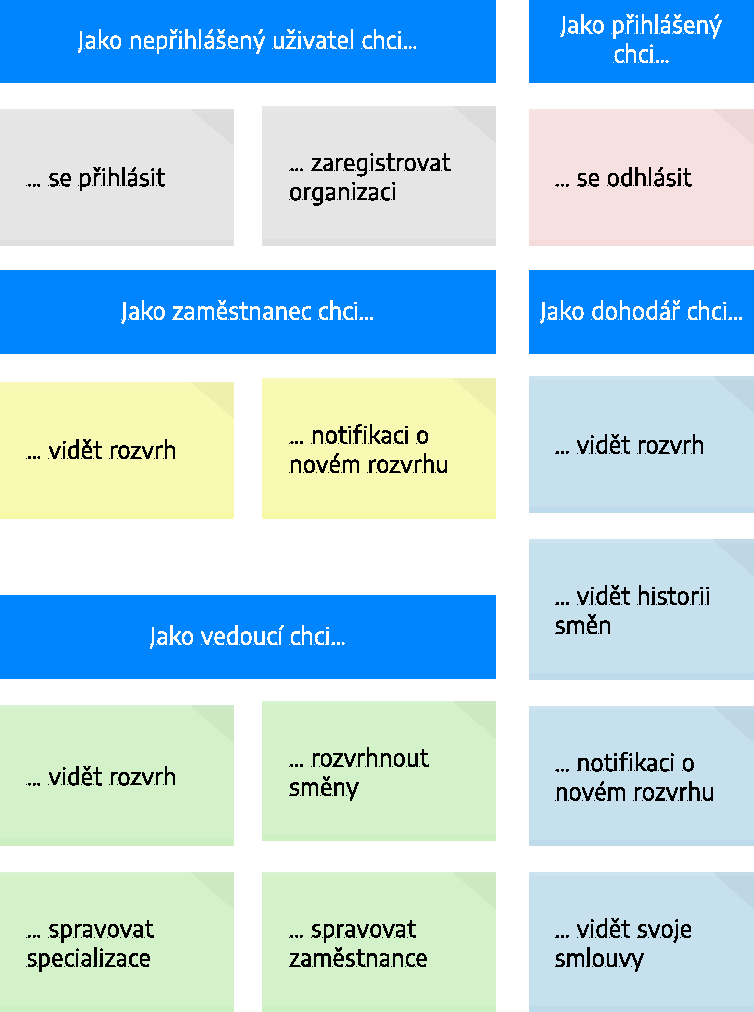
\includegraphics[scale=0.8]{user-stories.pdf}
	\caption{Zjednodušený storyboard}
	\label{fig:user-stories}
\end{figure}

% \begin{figure}[h!]
% \input{img/accounts-module.pdf_tex}
%
% 	\caption{Případy užití pro správu uživatelských účtů}
% 	\label{fig:uc-account}
% \end{figure}
%
% \begin{figure}[p!]
% 		\input{img/uc-dohoda.pdf_tex}
% 		\caption{Případy užití pro dohodáře}
% 		\label{fig:uc-employee}
% \end{figure}


\newpage

\chapter{Výběr technologií}
Při výběru technologií pro tento projekt hrály kromě samotných požadavků na tuto aplikaci roli i zkušenosti a preference autorky, konkrétní výběr byl tedy zkreslen i subjektivním hlediskem.

\section{Technologie pro uživatelské rozhraní}

Přestože jako téma této práce byla určena mobilní aplikace, a tedy již tento výběr neprobíhal, v~případě, že by byla aplikace implementována v~produkčním prostředí, připadaly by v~úvahu nejméně dva přístupy -- mobilní nebo webová aplikace.

\subsection{Webová aplikace}
Pro použití webové aplikace hovoří fakt, že webové aplikace není třeba žádným způsobem instalovat a stačí prosté zadání adresy do internetového prohlížeče. Aplikace je z~podstaty věci multiplatformní, neboť ji lze zobrazit v libovolném internetovém prohlížeči, tedy jak na počítači, tak na mobilním zařízení (jedná-li se o responzivní aplikaci, může být i použití webové aplikace na mobilním zařízení uživatelsky přívětivé). Nevýhodou tohoto přístupu jsou omezené možnosti při implementace offline režimu a rovněž i to, že z hlediska rychlosti se nativním mobilním aplikacím nevyrovnají.


\subsection{Mobilní aplikace}

Oproti responzivnímu webu mají nativní aplikace výhodu, že mohou jednoduše přistupovat k API, které poskytuje samotné zařízení, na kterém jsou nainstalované, tedy mohou snadno získat přístup k fotoaparátu či poloze zařízení. Dále lze na zařízení jednoduše přijímat notifikace, i když je aplikace na pozadí. Nativní aplikace mohou být vhodné i pro použití v offline režimu (použitím lokální databáze).

Pro uživatele mají tu nevýhodu, že se musí instalovat na zařízení (s~tím souvisí i o~něco složitější způsob distribuce). V~případě, že je možné zveřejnit aplikaci v~obchodech (Google Play, AppStore), musí projít schvalovacím procesem, což může trvat několik dní a nemusí být vždy úspěšné, pro Google Play např. v~případě, že aplikace obsahuje nevhodný obsah, narušuje ničí autorská práva nebo třeba nevhodným způsobem zpracovává osobní údaje svých uživatelů. Rovněž je třeba uvádět, jaká oprávnění aplikace pro přístup ke mobilním API (SMS, kontakty, poloha, soubory) požaduje. \cite{google2021policy}.

Při výběru konkrétního způsobu implementace mobilní aplikace pak existuje několik dalších rozhodovacích situací, především~výběr podporované platformy (iOS, Android) nebo způsob vývoje (pro jednu platformu, multiplatformní, hybridní).

\subsubsection{Platforma}
Na trhu s~mobilními zařízeními jsou dvě dominantní platformy, a to Android (podíl na trhus~chytrými telefony celosvětově 72~\%) a iOS (podíl na trhu 27,5~\%) \cite{statcounter2021mobile}. Aplikace lze připravovat přímo pro danou platformu, případně multiplatformně.


\paragraph{Multiplatformní vývoj}
Multiplatformní vývoj umožňuje nasazení jedné aplikace na více platformách, přičemž pro všechny platformy mají aplikace sdílený kód, jádro aplikace tedy není třeba duplikovat, což je jejich nespornou výhodou, navíc to může i snížit náklady na vývoj.

Problémem je přístup k~aplikačnímu rozhraní a hardwaru daného zařízení, omezené možnosti při používání knihoven specifických pro platformu nebo složitější vývoj uživatelského rozhraní tak, aby odpovídalo konvencím pro všechny platformy. \cite{manchanda2020where}   Používají se frameworky jako Flutter (jazyk Dart), React Native (JavaScript) nebo Xamarin (C\#).

\paragraph{Vývoj pro jednu platformu}
U vývoje na jednu platformu lze předpokládat, že bude možné používat všechny součásti zařízení naplno. Co se přístupu k hardwaru, výkonu a uživatelského prožitku týče, mají nativní aplikace nad multiplatformními jasnou převahu, jejich vývoj je však až dvakrát dražší. \cite{dennis2018native}


\subsubsection{Programovací jazyk}
Pro nativní vývoj na platformu Android lze vybrat nejméně ze tří možností, a to C/C++, Javy a Kotlinu. Toto rozhodování může v~této době u~nových projektů probíhat spíše pouze v teoretické rovině, neboť oficiální podporu ze strany Googlu má nejmodernější jazyk Kotlin.

Mezi hlavní výhody Kotlinu oproti jiným variantám patří null-safety (tedy bezpečné volání na objektech, které mohou nabývat hodnotu \texttt{null}), coroutines (odlehčená verze vláken pro asynchronní operace) nebo Kotlin Extensions (knihovny nejrůznějších funkcí usnadňující vývoj, a to jak obecně, tak i specificky pro platformu Android). \cite{android2021kotlin}


\subsection{Shrnutí}

Jako nejvhodnější by se v~případě produkčního nasazení této aplikace jevilo zkombinovat oba přístupy, tedy mít uživatelské rozhraní jak ve formě webové aplikaci, tak mít i podpůrnou mobilní aplikaci. Tento přístup byl také zvolen v případě většiny podobných řešení (viz podkapitolu \ref{sec:existing}). Zde byla implementována pouze jedna část, a to mobilní aplikace, neboť důraz byl kladen především na pohodlí zaměstnanců, kteří chtějí mít svůj rozvrh po ruce co nejrychleji. Pokud by naopak bylo prioritou vytvořit rozhraní přívětivé pro zobrazení přehledu o celkovém rozvrhu všech zaměstnanců, které vyžaduje větší rozlišení obrazovky, dávalo by větší smysl implementovat nejprve webové rozhraní.

Mobilní aplikace bude vyvinuta jako nativní Android aplikace, tento výběr je zkreslen zkušenostmi autorky, v~produkčním prostředí by bylo žádoucí uživatele iOS nediskriminovat a aplikaci jim také nabídnout, z~tohoto důvodu by bylo vhodné zvážit použití nějakého multiplatformního frameworku, rozhodující by byly plány na budoucí vývoj, případně i~finance. Pro vývoj se použije programovací jazyk Kotlin, protože se jedná o moderní programovací jazyk, který je pro vývoj na danou platformu nejvhodnější.


\section{Backendová technologie}

\subsection{Webový framework}

Webové frameworky, tj. knihovny zdrojových kódů připravené pro tvorbu webů (především jejich serverové strany), se standardně používají pro zjednodušení vývoje a nasazení aplikací. Ať už jsou napsány v~libovolném programovacím jazyce (může jít např.~o~PHP, Java, Ruby nebo Python), standardními součástmi jsou dle \cite{docforge2014web} perzistence dat, autentizace uživatelů, správa session nebo šablony pro uživatelské rozhraná. Společnou mají rovněž podporu pro architekturu MVC\footnote{Model-View-Controller}.

Z~množství variant, které se nabízejí, byl zvolen framework Ruby on Rails (v~jazyce Ruby), a to především z~důvodu jeho zásad Don't Repeat Yourself (kód by měl být znovupoužitelný, bez zbytečného opakování) a Convention Over Configuration (webová aplikace je nakonfigurována dle konvencí, a vývojář tak nemusí trávit čas psaním konfiguračních souborů) \cite{rails2020}, které slibují výrazné usnadnění vývoje.

% \subsubsection{Model-View-Controller}

% \paragraph{Model (model)}
%
% Model je část aplikace, která reprezentuje business data aplikace a jejich logiku, v~sobě zahrnuje jak perzistentní data, tak operace s~nimi. V Rails jsou modely implementovány jako ActiveRecord, který zde slouží jako ORM\footnote{Object-Relation Mapper} framework, stará se o~validace objektů před jejich uložením do databáze, mapuje asociace mezi objekty a~zprostředkovává databázové operace (není tak třeba psát žádné SQL dotazy -- o vytvoření databáze a~operace s~ní se starají Rails samy).
%
% \subsection{View (pohled)}
%
% Pohled je zodpovědný za vykreslování uživatelského rozhraní, především za generování HTML kódu stránky (základem jsou šablony, do nichž se doplňují konkrétní data z~modelů).
%
% \subsection{Controller (řadič)}
%
% Controller je část aplikace, která je zodpovědná za zpracování požadavků -- když přijde na controller požadavek, naleznou se odpovídající data v modelu a view je zobrazí.


% \subsubsection{Ruby On Rails}

\subsection{Aplikační rozhraní}

Pro komunikaci s~dalšími aplikacemi (zde především pro komunikaci klienta se serverem) musí aplikace veřejně poskytnout své aplikační rozhraní, přičemž za tímto účelem existuje několik variant, které jsou vhodné pro různé případy (např.~REST, SOAP, GraphQL, gRPC). Tyto způsoby implementace se mohou od sebe odlišovat formátem přenosu (binární, textový) nebo protokolem (HTTP i~jiné).

Pro účely tohoto projektu se jako optimální varianta jeví použití REST API, a to vzhledem k~velmi dobré podpoře ze strany webového frameworku bez nutnosti rozšiřování o~další knihovny (konkrétně Ruby on Rails podporují vytváření cest na základě konvencí – pokud tak controller definuje metodu \texttt{update}, automaticky se vytvoří endpoint \texttt{PUT/PATCH /resources/:id}, případně lze cesty definovat v~souboru \texttt{config/routes.rb} a provolat tak libovolnou akci v~libovolném controlleru).

V některých případech by bylo vhodnější použít pro komunikaci jiný prostředek (především v~případě volání výpočtů na serveru), např.~RPC (gRPC, XML-RPC, JSON-RPC či jinou konkrétní implementaci), neboť zde nedochází k~přenosu zdrojů (způsob využití REST API, který vyplývá z~definice), ale pouze k~výpočtům na vzdáleném serveru. Toto by ale vytvořilo problémy při nasazení aplikace na PaaS službách (např. Heroku), proto bylo zvoleno řešení, které sice není z~hlediska architektury tou nejlepší volbou, ale je jednodušší na použití.

\subsection{Databáze}

Rozhodování ohledně použité databáze se může týkat způsobu uložení dat (relační nebo NoSQL) a samotného DBMS (systém správy báze dat). Je třeba se rozhodnout, zda v~projektu bude použita relační či NoSQL databáze. Relační databáze přitom jsou vhodné na ukládání dat se statickou strukturou, kdežto NoSQL databáze mohou být flexibilnější, co se ukládání dat týče.  \cite{geeks2020difference} Pro účely tohoto projektu byla zvolena relační databáze, a to z~důvodu předem určené struktury dat a taktéž proto, že jde o technologii, která má dobrou podporu, a to i ze strany webových frameworků. Upřednostněna tedy byla známá technologie. Jako konkrétní systém správy báze dat byl zvolen Postgres.


\subsection{Shrnutí}

Aplikace bude vyvinuta ve webovém frameworku Ruby on Rails, a to vzhledem k~tomu, že jde o~rozšířený framework, který slibuje jednoduchou konfiguraci. S~vnějškem bude tato aplikace komunikovat prostřednictvím REST API vzhledem k~jednoduché implementaci a silné podpoře pro jeho využití. Použita bude relační databáze, konkrétně Postgres.

\section{Požadavky na kvalitu software}

Z~rozhodování v~této kapitole vyplynuly následující požadavky na kvalitu software:

\begin{enumerate}[label=\textbf{S\arabic*.}]
	\item Bude vyvinuta nativní Android aplikace v~jazyce Kotlin.
	\item Backend bude vyvinut ve webovém frameworku Ruby on Rails.
	\item Mobilní aplikace bude se serverem komunikovat přes jeho REST API.
	\item Bude použita databáze Postgres.
\end{enumerate}

% \subsection{UC1: Přihlásit se}
% \paragraph{Aktér:} Nepřihlášený uživatel
% \paragraph{Hlavní scénář:}
% 	\begin{enumerate}
% 		\item Systém zobrazí obrazovku Přihlášení (obr.~\ref{fig:signin})
% 		\item Nepřihlášený uživatel vyplní uživatelské jméno a heslo, klikne na tlačítko Přihlásit se.
% 		\item Systém zobrazí obrazovku Hlavní stránka. Uživatel je přihlášen.
% 	\end{enumerate}
%
% 	\begin{figure}[h]
% 		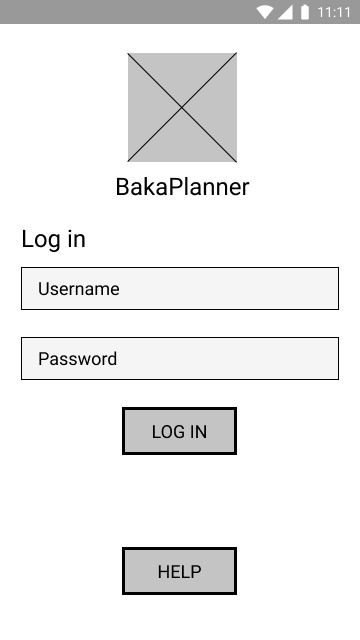
\includegraphics[scale=.35]{img/sign_in_form.png}
% 		\caption{Obrazovka Přihlášení}
% 		\label{fig:signin}
% 	\end{figure}
%
% \paragraph{Alternativní scénář a) (uživatel nezadá uživatelské jméno a/nebo heslo):}
%
% 	\begin{enumerate}[label=\arabic*a]
% 		\setcounter{enumi}{2}
% 		\item Systém zobrazí chybovou hlášku \uv{Vyplňte prosím uživatelské jméno/heslo}.
% 	\end{enumerate}
%
% \paragraph{Alternativní scénář b) (uživatel zadá špatné přihlašovací údaje)}
%
% 	\begin{enumerate}[label=\arabic*b]
% 		\setcounter{enumi}{2}
% 		\item Systém zobrazí chybovou hlášku \uv{Špatné uživatelské jméno nebo heslo}.
% 	\end{enumerate}
%
% \paragraph{Alternativní scénář c) (uživatel je offline)}
%
% 	\begin{enumerate}[label=\arabic*c]
% 		\setcounter{enumi}{2}
% 		\item Systém zobrazí hlášku \uv{Nejste připojeni k~internetu.}
% 	\end{enumerate}
% \newpage
% \subsection{UC2: Odhlásit se}
% \paragraph{Aktér:} Přihlášený uživatel
% \paragraph{Hlavní scénář:}
% \begin{enumerate}
% 	\item Uživatel klikne na záložku Profil.
% 	\item Systém zobrazí obrazovku Profil (obr.~\ref{fig:profile}).
% 	\item Uživatel stiskne tlačítko Odhlásit se.
% 	\item Systém odhlásí uživatele. Zobrazí se obrazovka Přihlášení
% \end{enumerate}
%
% \begin{figure}[h]
% 	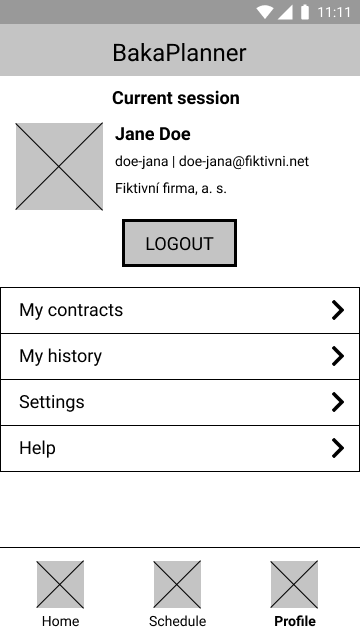
\includegraphics[scale=.35]{img/main-profile.png}
% 	\caption{Obrazovka Profil}
% 	\label{fig:profile}
% \end{figure}
%
% \paragraph{Alternativní scénář a) (uživatel je offline)}
%
% 	\begin{enumerate}[label=\arabic*a]
% 		\setcounter{enumi}{3}
% 		\item Systém zobrazí hlášku \uv{Nejste připojeni k~internetu.}
% 	\end{enumerate}
%
% \newpage
% \subsection{UC3: Zobrazit rozvrh směn}
% \paragraph{Aktér:} Zaměstnanec
% \paragraph{Hlavní scénář:}
% \begin{enumerate}
% 	\item Uživatel klikne na záložku Rozvrh směn.
% 	\item Systém zobrazí obrazovku Rozvrh směn (obr.~\ref{fig:schedule}), v~níž je seznam uživateli přiřazených směn.
% \end{enumerate}
%
% \begin{figure}[h]
% 	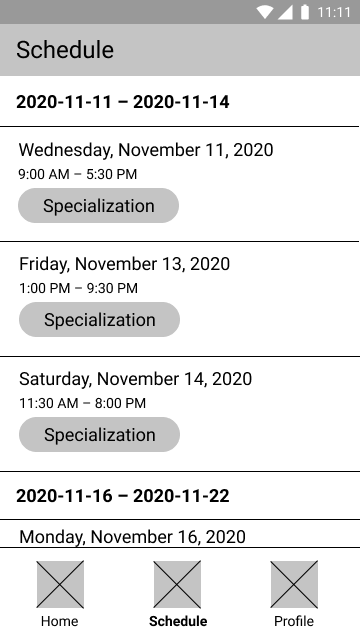
\includegraphics[scale=.35]{img/main-schedule.png}
% 	\caption{Obrazovka Rozvrh směn}
% 	\label{fig:schedule}
% \end{figure}
%
% \paragraph{Alternativní scénář a) (uživatel je offline a data nejsou uložena lokálně):}
% \begin{enumerate}[label=\arabic*a]
% 	\setcounter{enumi}{1}
% 	\item Systém zobrazí hlášku \uv{Nejste připojeni k~internetu.}
% \end{enumerate}
%
% \paragraph{Alternativní scénář b) (rozvrh směn je prázdný):}
% \begin{enumerate}[label=\arabic*b]
% 	\setcounter{enumi}{1}
% 	\item Systém zobrazí hlášku \uv{Váš rozvrh směn je prázdný.}
% \end{enumerate}
%
% \newpage
% \subsection{UC4: Zobrazit detail směny}
% \paragraph{Aktér:} Zaměstnanec
% \paragraph{Předpoklady:} Je zobrazen přehled směn (např. obrazovka Rozvrh směn nebo Historie).
% \paragraph{Hlavní scénář:}
% \begin{enumerate}
% 	\item Uživatel klikne na konkrétní směnu ze seznamu.
% 	\item Systém zobrazí obrazovku Detail směny (obr.~\ref{fig:shift-detail}).
% \end{enumerate}
%
% \begin{figure}[h!]
% 	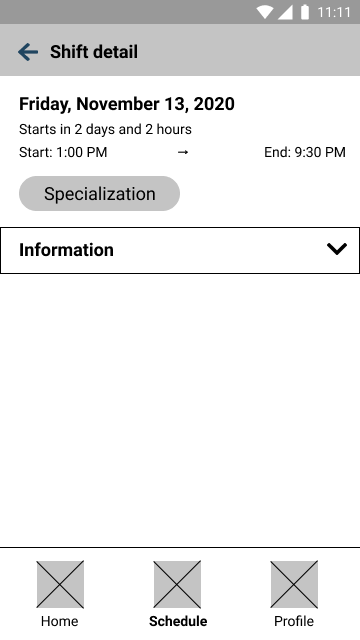
\includegraphics[scale=.35]{img/shift-detail.png}
% 	\caption{Obrazovka Detail směny}
% 	\label{fig:shift-detail}
% \end{figure}
% 	%
% 	% \begin{tabular}{|p{0.2\linewidth}|p{0.02\linewidth}p{0.7\linewidth}|}
% 	% 	\hline
% 	% 	\multicolumn{3}{|c|}{Případ užití: \textbf{Zobrazit detail směny}}\\
% 	% 	\hline
% 	% 	Předpoklady: & \multicolumn{2}{|l|}{Zobrazit osobní rozvrh směn nebo Zobrazit seznam volných směn}\\
% 	% 	\hline
% 	% 	Hlavní scénář: & 1. & Uživatel klikne na konkrétní směnu.\\
% 	% 	& 2. & Systém zobrazí obrazovku Detail směny. \\
% 	% 	\hline
% 	% 	Vedlejší scénáře: & 1a & Uživatel je offline a žádná data nejsou dostupná lokálně. Systém zobrazí hlášku \uv{Zkontrolujte připojení k~internetu.} \\
% 	% 	\hline
% 	% \end{tabular}
%
% % \begin{figure}
% % 	\input{img/use-cases.pdf_tex}
% % 	\caption{Diagram případů užití}
% % 	\label{fig:usecase}
% % \end{figure}
% \newpage
% \subsection{UC5: Zobrazit přehled nejbližších směn}
% \paragraph{Aktér:} Zaměstnanec
% \paragraph{Hlavní scénář:}
% \begin{enumerate}
% 	\item Uživatel otevře aplikaci nebo klikne na záložku Domů.
% 	\item Systém zobrazí Domovskou obrazovku (obr.~\ref{fig:home}) s~přehledem nejbližších směn.
% \end{enumerate}
%
%
% \paragraph{Alternativní scénář a) (uživatel je offline a data nejsou uložena lokálně):}
% \begin{enumerate}[label=\arabic*a]
% 	\setcounter{enumi}{1}
% 	\item Systém zobrazí hlášku \uv{Nejste připojeni k~internetu}.
% \end{enumerate}
%
% \paragraph{Alternativní scénář b) (rozvrh směn je prázdný):}
% \begin{enumerate}[label=\arabic*b]
% 	\setcounter{enumi}{1}
% 	\item Systém zobrazí hlášku \uv{Už nemáte nic naplánováno}.
% \end{enumerate}
%
% \begin{figure}[h]
% 	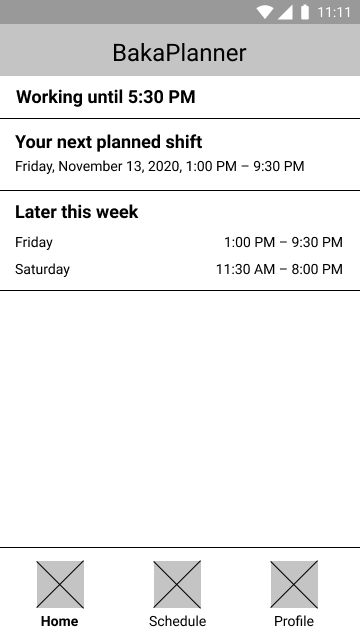
\includegraphics[scale=.35]{img/main-home.png}
% 	\caption{Domovská obrazovka}
% 	\label{fig:home}
% \end{figure}
% \newpage
% \subsection{UC6: Zobrazit historii odpracovaných směn}
% \paragraph{Aktér:} Zaměstnanec
% \paragraph{Předpoklady:} Je zobrazena obrazovka Profil.
% \paragraph{Hlavní scénář:}
% \begin{enumerate}
% 	\item Uživatel klikne na tlačítko \uv{Historie}
% 	\item Systém zobrazí obrazovku Historie (obr.~\ref{fig:history}), v~níž je seznam uplynulých směn uživatele.
% \end{enumerate}
%
% \begin{figure}[h!]
% 		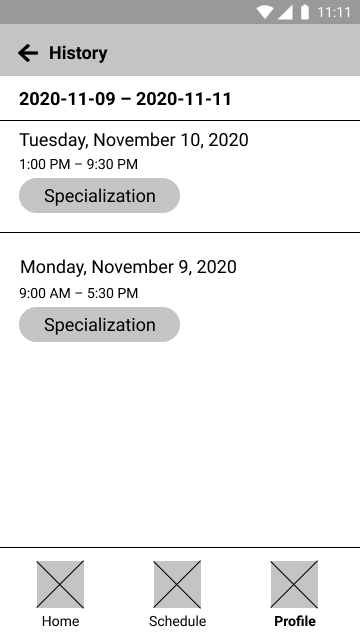
\includegraphics[scale=.35]{img/history.png}
% 		\caption{Obrazovka Historie}x
% 		\label{fig:history}
% \end{figure}
%
% \paragraph{Alternativní scénář a) (uživatel je offline a data nejsou uložena lokálně):}
% \begin{enumerate}[label=\arabic*a]
% 	\setcounter{enumi}{1}
% 	\item Systém zobrazí hlášku \uv{Nejste připojeni k~internetu}.
% \end{enumerate}
%
% \paragraph{Alternativní scénář b) (seznam směn je prázdný):}
% \begin{enumerate}[label=\arabic*b]
% 	\setcounter{enumi}{1}
% 	\item Systém zobrazí hlášku \uv{Historie vašich směn je prázdná}.
% \end{enumerate}
%
% \newpage
% \subsection{UC7: Zobrazit přehled smluv}
% \paragraph{Aktér:} Zaměstnanec
% \paragraph{Předpoklady:} Je zobrazena obrazovka Profil.
% \paragraph{Hlavní scénář:}
% \begin{enumerate}
% 	\item Uživatel klikne na tlačítko \uv{Smlouvy}
% 	\item Systém zobrazí obrazovku Smlouvy (obr.~\ref{fig:contracts}), v~níž je seznam aktuálních i neaktuálních smluv uživatele.
% \end{enumerate}
%
% \begin{figure}[h!]
% 		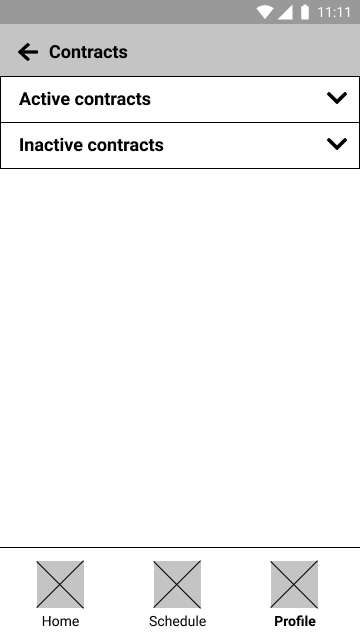
\includegraphics[scale=.35]{img/contracts.png}
% 		\caption{Obrazovka Smlouvy}
% 		\label{fig:contracts}
% \end{figure}
%
% \paragraph{Alternativní scénář a) (uživatel je offline a data nejsou uložena lokálně):}
% \begin{enumerate}[label=\arabic*a]
% 	\setcounter{enumi}{1}
% 	\item Systém zobrazí hlášku \uv{Nejste připojeni k~internetu}.
% \end{enumerate}
%
% \newpage
% \subsection{UC8: Zobrazit seznam volných směn}
% \paragraph{Aktér:} Zaměstnanec na dohodu
% \paragraph{Hlavní scénář:}
% \begin{enumerate}
% 	\item Uživatel klikne na záložku Směny.
% 	\item Systém zobrazí obrazovku Volné směny (obr.~\ref{fig:unassigned}) se seznamem všech směn, které si může uživatel zapsat do rozvrhu.
% \end{enumerate}
%
% \begin{figure}[h!]
% 		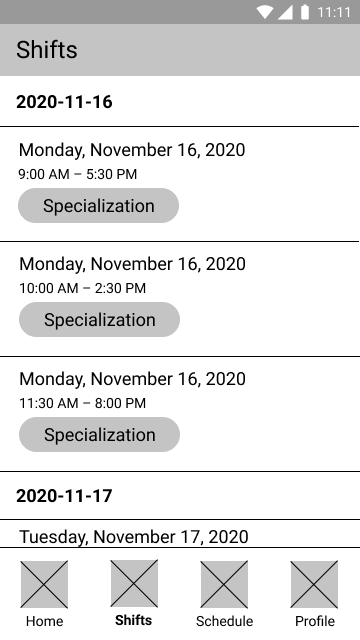
\includegraphics[scale=.35]{img/main-shifts.png}
% 		\caption{Obrazovka Volné směny}
% 		\label{fig:unassigned}
% \end{figure}
%
% \paragraph{Alternativní scénář a) (uživatel je offline):}
% \begin{enumerate}[label=\arabic*a]
% 	\setcounter{enumi}{1}
% 	\item Systém zobrazí hlášku \uv{Nejste připojeni k~internetu}.
% \end{enumerate}
%
% \paragraph{Alternativní scénář b) (seznam volných směn je prázdný):}
% \begin{enumerate}[label=\arabic*b]
% 	\setcounter{enumi}{1}
% 	\item Systém zobrazí hlášku \uv{Žádné volné směny nebyly nalezeny.}.
% \end{enumerate}
%
%
% \newpage
% \subsection{UC9: Zapsat se na volnou směnu}
% \paragraph{Aktér:} Zaměstnanec na dohodu
% \paragraph{Předpoklady:} Je zobrazena obrazovka Detail směny (obr.~\ref{fig:shift-detail-up}) pro směnu, kterou si uživatel může zapsat\footnote{Bude tedy třeba ošetřit, aby se možnost zápisu na směnu nabídla pouze v~případě, že se směna nepřekrývá s~žádnou ze směn v~rozvrzích daného zaměstnance.}.
% \paragraph{Hlavní scénář:}
% \begin{enumerate}
% 	\item Uživatel klikne na tlačítko Zapsat směnu.
% 	\item Systém zobrazí obrazovku Vybrat rozvrh (obr.~\ref{fig:pick-schedule}) se seznamem všech rozvrhů, do nichž lze směnu zapsat.
% 	\item Uživatel ze seznamu vybere rozvrh, do nějž chce směnu zapsat.
% 	\item Systém zobrazí zprávu \uv{Směna byla zapsána do~rozvrhu.} Směna je zapsána do osobního rozvrhu zaměstnance.
% \end{enumerate}
%
% \begin{figure}[h!]
% 	\centering
% 	\begin{subfigure}{.45\textwidth}
% 		\centering
% 		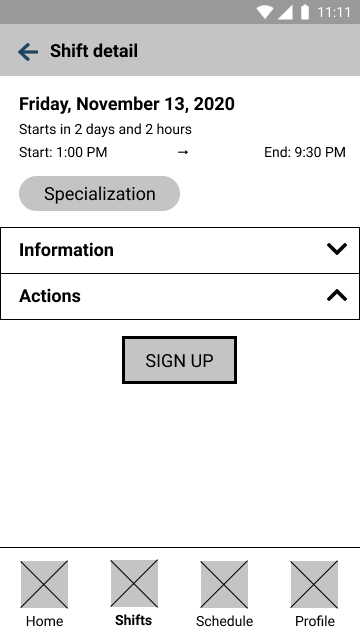
\includegraphics[scale=.35]{img/shift-detail-up.png}
% 		\caption{Obrazovka Detail směny}
% 		\label{fig:shift-detail-up}
% 	\end{subfigure}
% 	\begin{subfigure}{.45\textwidth}
% 		\centering
% 		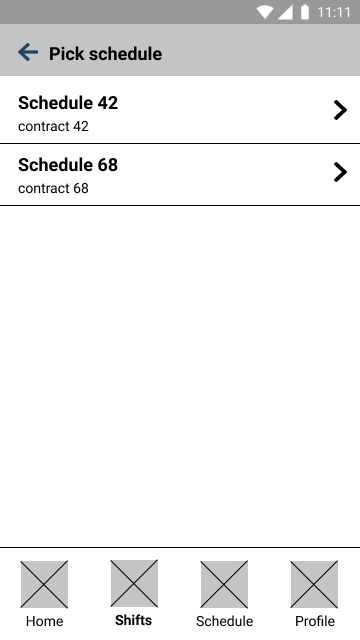
\includegraphics[scale=.35]{img/pick-schedule.png}
% 		\caption{Obrazovka Vybrat rozvrh}
% 		\label{fig:pick-schedule}
% 	\end{subfigure}
% 	\caption{Obrazovky pro UC9: Zapsat se na volnou směnu}
% \end{figure}
%
%
% \paragraph{Alternativní scénář a) (uživatel je offline a data nejsou uložena lokálně):}
% \begin{enumerate}[label=\arabic*a]
% 	\setcounter{enumi}{1}
% 	\item Systém zobrazí hlášku \uv{Nejste připojeni k~internetu}.
% \end{enumerate}
%
%
% \newpage
% \subsection{UC10: Zrušit zápis na směnu}
% \paragraph{Aktér:} Zaměstnanec na dohodu
% \paragraph{Předpoklady:} Je zobrazena obrazovka Detail směny (obr.~\ref{fig:shift-detail-remove}) pro směnu, jejíž zápis uživatel může zrušit.
% \paragraph{Hlavní scénář:}
% \begin{enumerate}
% 	\item Uživatel klikne na tlačítko \uv{Odebrat z~rozvrhu}.
% 	\item Systém zobrazí dialog Jste si jisti? (obr.~\ref{fig:shift-remove-confirm}).
% 	\item Uživatel potvrdí smazání.
% 	\item Systém zobrazí zprávu \uv{Směna byla odstraněna z~rozvrhu.} Směna je odstraněna z~rozvrhu.
% \end{enumerate}
%
% \begin{figure}[h!]
% 	\centering
% 	\begin{subfigure}{.45\textwidth}
% 		\centering
% 		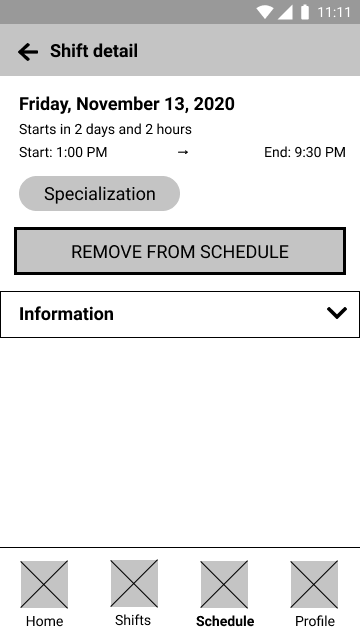
\includegraphics[scale=.35]{img/shift-detail-remove.png}
% 		\caption{Obrazovka Detail směny}
% 		\label{fig:shift-detail-remove}
% 	\end{subfigure}
% 	\begin{subfigure}{.45\textwidth}
% 		\centering
% 		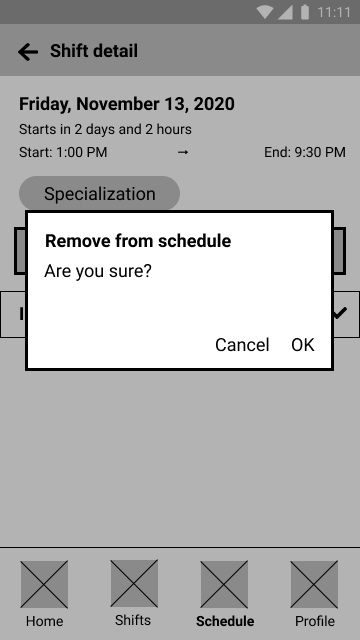
\includegraphics[scale=.35]{img/shift-detail-remove-confirm.png}
% 		\caption{Dialog Jste si jisti?}
% 		\label{fig:shift-remove-confirm}
% 	\end{subfigure}
% 	\caption{Obrazovky pro UC10: Zrušit zápis na směnu}
% \end{figure}
%
%
% \paragraph{Alternativní scénář a) (uživatel je offline a data nejsou uložena lokálně):}
% \begin{enumerate}[label=\arabic*a]
% 	\setcounter{enumi}{3}
% 	\item Systém zobrazí hlášku \uv{Nejste připojeni k~internetu}.
% \end{enumerate}
%
% \paragraph{Alternativní scénář b) (uživatel nepotvrdí smazání):}
% \begin{enumerate}[label=\arabic*b]
% 	\setcounter{enumi}{3}
% 	\item Systém schová dialog Jste si jisti? (obr.~\ref{fig:shift-remove-confirm}) a zobrazí obrazovku Detail směny (obr.~\ref{fig:shift-detail-remove}).
% \end{enumerate}


\chapter{Rozvrhování směn}
Problém plánování směn je jedním z~rozvrhovacích problémů\footnote{Dalšími takovými problémy jsou např.~sestavování školních rozvrhů nebo jízdních řádů.}, obecně se považuje velmi komplexní, a to i v~případě, že se řeší jen jeho zjednodušená verze (např. se vyhodnocuje jen jedno kritérium a schopnosti zaměstnanců jsou homogenní). V~rámci velkých organizací lze složitost tohoto problému snížit například tím, že na sobě nezávislé části mají samostatný rozvrh (např. v~nemocnici je rozvrh ostrahy nezávislý na rozvrhu lékařů na patologii). Teoretických problémů, které byly popsány v literatuře a které se týkají rozvrhování pracovních sil, existuje více druhů dle podmínek a prostředí, jehož se bezprostředně týkají, poznatky ovšem lze použít pro obecný problém rozvrhování směn, i~když se týkají např.~problému rozvrhování zdravotních sester.

Přístupů, jak problém rozvrhování personálu řešit, existuje celá řada, například lze rozvrh sestavovat centrálně, v~kooperaci se zaměstnanci nebo nějakým hybridním způsobem; rozvrh může být sestaven člověkem (na papír, v~tabulkovém editoru, \ldots) či automaticky.

Výzkum tohoto problému se zaměřuje především na vývoj efektivních přibližných metod řešení. \cite{adamuthe2012tabu} Řešení totoho rozvrhovacího problému lze automatizovat více způsoby, které jsou vhodné v~závislosti na jeho formulaci (pro více viz podkapitolu~\ref{sec:clasif}) -- v~jednoduchém případě může být možné ho interpretovat tak, aby odpovídal problému již známému a řešitelnému standardními metodami\footnote{Může se jednat např. o~lineární programování, které nalezne optimální řešení, ovšem jen jedná-li se o~méně komplexní problémy (např. je obtížné formulovat všechny zbytné podmínky pouze jako lineární funkce)}, dalším je heuristika, která umožňuje řešení komplexnějších problémů, avšak ne vždy zaručuje nalezení optimálního řešení. \cite{blochliger2004modeling}

V~této kapitole bude podrobněji popsán proces rozvrhování směn, rozhodující proměnné a vybrané teoretické metody, jak tento problém lze řešit a dále způsob řešení, který byl na jejich základě poznatků z~tohoto vyplývajících implementován v~rámci této práce.

\section{Proces rozvrhování směn}
Dle \cite{ernst2004staff} lze proces rozvrhování rozdělit na několik částí, které na sebe mohou, ale nemusí nutně navazovat. Konkrétně se jedná o:
\begin{enumerate}
	\item předpovídání poptávky po personálu;
	\item rozvrhování volných dnů;
	\item rozvrhování směn;
	\item rozvrhování prací;
	\item rozdělení úkolů;
	\item přidělení osob.
\end{enumerate}

\section{Definice problému}

Rozvrhování směn obecně řeší problém, že organizace má k~dispozici $N$~zaměstnanců, které je třeba rozdělit do $S$ směn v~$D$~pracovních dnech, a~to na základě sady podmínek, které se liší dle charakteru provozu.

\section{Klasifikace}
\label{sec:clasif}

Každý jednotlivý problém rozvrhování směn se od sebe může lišit, \cite{de2011categorisation} jako příklad uvádí:

\subparagraph{Základní charakteristiky}
Na jaké úrovni detailu se definují typy směn, schopnosti nebo pokrytí? Jak flexibilní jsou parametry? Jsou rozvrhy cyklické?

\paragraph{Fixní a flexibilní rozvrhování}
Rozvrhování je fixní (cyklické), pokud zaměstnanec pracuje v $n$-týdenních cyklech a jeho rozvrh se periodicky opakuje (případně pokud je stejný v~každém týdnu). Naproti tomu stojí rozvrhování flexibilní, v~němž taková pravidelnost neexistuje. \cite{burke2004state}

\subparagraph{Cíle}
Je hlavním cílem optimalizovat, nebo jenom nějak rozhodnout? Optimalizuje se dle podmínek, počtu personálu nebo něčeho jiného?

\subparagraph{Podmínky}
Kolik je podmínek? Jakého jsou podmínky typu? Jaké podmínky jsou zbytné a jaké nezbytné?

\subparagraph{Velikost problému}
Na jak dlouho se plánuje? Pro kolik zaměstnanců se rozvrh plánuje? Kolik je typů směn?


\section{Podmínky}
\label{sec:constraints}
Rozvrhování směn závisí na takovém množství podmínek, že je obvykle není možné splnit všechny, proto se také často musí před samotným řešením problému rozdělit na nezbytné~(hard, značeno $H_i$, musí být splněny vždy) a~zbytné~(soft, značeno $S_i$, jejich splnění je žádoucí). \cite{todorovic2012bee} Pro každou podmínku, obzláště zbytnou, je vhodné stanovit její váhu, například tak, že nezbytné podmínky mají váhu v~řádu vyšších stovek (mezi 500 a 1000) a zbytné podmínky mají váhu řádově menší (mezi 50 a 150). \cite{buyukozkan2014applicability}

Podmínky se mohou týkat například sekvence činností (např. po náročné chirurgické operaci může následovat pouze administrativní činnost nebo po směně nemůže následovat 12 hodin další směna), počtu (např. zaměstnanec pracuje týdně~$ 40~\pm 8~\mbox{h}$), nekompatibilních stavů (např. Alice nechce pracovat s~Bobem) nebo nezbytných činností (např.~je v~daném dni naplánována náročná operace srdce). Lze je rozdělit na globální, jejichž posouzení vyžaduje celkovou znalost řešení (Je na každé směně někdo?), a lokální, na jejichž verifikaci stačí pohled na vlastní podmnožinu řešení (Má tento zaměstnanec volný víkend?). Toto rozdělení je naznačeno na obr.~\ref{fig:constraints}, nezbytné činnosti však nelze rozdělit z~tohoto pohledu jednoznačně (mohou se týkat jak celého rozvrhu, tak jeho části). \cite{blochliger2004modeling}

\begin{figure}[h]
	\input{img/constraints.pdf_tex}
	\caption{Rozdělení podmínek dle jejich rozsahu}
	\label{fig:constraints}
\end{figure}

\newpage
\section{Interpretace řešení}
Řešení tohoto problému lze interpretovat jako trojrozměrnou binární matici $\boldsymbol{R}$, jejímiž parametry jsou zaměstnanec ($\forall i \in E$), den ($\forall j \in T$) a vypsaná směna ($\forall k \in S$), jednotlivé hodnoty $R_{ijk}$ jsou určeny funkcí \ref{eq:3dmatrix}. \cite{vaclavik2016roster}

\begin{equation}
	\label{eq:3dmatrix}
	R_{ijk} =
	\begin{cases}
		1, & \mbox{zaměstnanci $i$ je v den $j$ přiřazena směna $k$,} \\
		0, & \mbox{jinak.}\\
	\end{cases}
\end{equation}

Příklad toho, jak lze řešení popsané ve funkci~\ref{eq:3dmatrix} interpretovat ve formě tabulky, je v~tab.~\ref{tab:interpretation}
\begin{table}[h]
	\input{tables/interpretation-example.tex}
	\caption{Interpretace řešení}
	\label{tab:interpretation}
\end{table}

Dále může být rozvrh směn interpretován jako vektor $\boldsymbol{x} = (x^1, x^2,~\ldots,~x^N)$, kde každé přiřazení $x^m = (i, j, k)$ značí, že zaměstnanci $i$ je ve dni~$j$ přiřazena $k$-tá směna. \cite{awadallah2015hybrid}

\section{Cílová funkce}
\label{sec:objective}
Cílová nebo také účelová funkce (angl. objective function) je taková funkce, jejíž hodnotu je cílem optimalizovat (minimalizovat nebo maximalizovat). V~případě rozvrhování směn se může jednat o funkce vyjadřující rovnoměrnost obsazení směn, cenu, porušené zbytné podmínky \cite{blochliger2004modeling} či počet kontaktů mezi zaměstnanci (důležitý např. v~případě epidemie) \cite{zucchi2020personnel}.

Například v~případě optimalizace na základě vážených podmínek dle podkapitoly \ref{sec:constraints} ji lze formulovat jako
\begin{equation}
	f(\boldsymbol{x}) = \sum_{s = 1}^n c_s \cdot g_s(\boldsymbol{x}),
\end{equation}
kde $\boldsymbol{x}$ je dané řešení, $n$ je počet zbytných podmínek, $c_s$ je váha~$s$-té~podmínky (také lze tento údaj chápat jako sankci za její porušení) a $g_s(\boldsymbol{x})$ je počet porušení $s$-té~podmínky v~řešení~$\boldsymbol{x}$. \cite{awadallah2015hybrid}
\newpage

\section{Vstupy}
Organizace má množinu zaměstnanců $M$, z~nichž každý zaměstnanec $m \in M$ má určenou množinu činností $Q_m$, které je kvalifikován vykonávat; podmnožině zaměstnanců $E \subseteq M$, $E = \{ 1, 2,~\ldots, e \}$ v~daném období může být rozvrhnuta směna. Každý zaměstnanec přitom v jednom čase může být pouze na jednom místě, mezi směnami by měl mít přestávku.

\begin{figure}[h]
	\input{img/problem-definition.pdf_tex}
	\caption{Ilustrace problému}
	\label{fig:definition}
\end{figure}

Rozvrh se vytváří na období $T = \{1, 2,~\ldots, t \}$ (typicky je toto období rozděleno na dny), v~každém dni jsou vypsány směny $S = \{ 1, 2,~\ldots, s\}$, které jsou charakterizovány např. časovým intervalem nebo požadovanou kvalifikací.

Byla použita některá z~metodik na předpovídání poptávky po personálu (viz podkapitolu \ref{sub:demand}), výsledkem je tabulka (viz např. \ref{tab:demand}), v~buňkách je potřebný počet zaměstnanců v~daném čase (poptávku může určit také rozmezí počtu zaměstnanců nebo to může být relativní veličina).

\begin{table}[h]
	\input{tables/demand-tabular.tex}
	\caption{Příklad týdenní poptávky}
	\label{tab:demand}
\end{table}

Dalším vstupem je tabulka s~nezbytnými (tab.~\ref{tab:hard}) a zbytnými (tab.~\ref{tab:soft}) požadavky, které mohou být ohodnocené.

\begin{table}[h]
	\begin{tabular}{|@{\makebox[3em][c]{${H}_{\rownumber}$}} |l|c|}
	\hline
	\multicolumn{1}{|@{\makebox[3em][c]{ID}} | l |}{ Požadavek } & Váha\\
	\hline
	Všechny směny musí být zaplněny. & 1000 \\
	{Každý pracovník může pracovat nejvýše jednu směnu denně.} & 1000 \\
	Ranní směna nemůže následovat po noční. & 1000\\
	\hline
	\end{tabular}

	\caption{Příklad nezbytných podmínek}
	\label{tab:hard}

\end{table}

\begin{table}[h]
	\begin{tabular}{|@{\makebox[3em][c]{${S}_{\rownumber}$}} |p{0.8\linewidth}|c|}
	\hline
	\multicolumn{1}{|@{\makebox[3em][c]{ID}} | l |}{ Požadavek } & Váha\\
	\hline
	{Jsou dodrženy požadavky zaměstnanců na volno.} & 100 \\
	{Dvojice zaměstnanců nechce pracovat společně.} & 50 \\
	Zaměstnanci mají alespoň dva volné víkendy za sebou & 50 \\
	\multicolumn{1}{|@{\makebox[3em][c]{$\vdots$ }} | c |}{ $\vdots$  } & $\vdots$ \\
	\hline
	\end{tabular}

	\caption{Příklad zbytných podmínek}
	\label{tab:soft}
\end{table}


\section{Lineární programování}
Úlohou lineárního programování\footnote{Termín programování zde souvisí se slovem program ve významu plán nebo rozvrh, nikoli s~počítačovými programy. } je nalézt vektor $\boldsymbol{x}^{\ast} \in \mathbb{R}^n$ optimalizující hodnotu cílové funkce mezi všemi vektory, které splňují danou soustavu lineárních rovnic a nerovnic (kterým se zpravidla říká omezující podmínky nebo omezení). \cite{matousek2006linearni}

\subsubsection{Celočíselné lineární programování}

Celočíselné lineární programování je pro rozvrhování směn vhodné v jed\-no\-du\-chých případech, např. když jsou pro všechny zaměstnance stanoveny stejné počty po sobě jdoucích pracovních dnů a volna nebo, jsou-li rozvrhovány směny v rámci dne, je den rozdělen na několik disjunktních úseků, navíc je stanoven počet po sobě následujích úseků, které tvoří jednu směnu. Pro každý časový úsek (den či část dne) je navíc stanoven minimální počet personálu. \cite{satheeshkumar2014linear} Cílem je optimalizovat počet zaměstnanců tak, aby byla minimální poptávka naplněna.

V~případě týdne, v~němž mají zaměstnanci 5 po sobě jdoucích pracovních dnů a 2 po sobě jdoucí dny volna, je rozdělení ilustrováno na obr. \ref{fig:linear}. Příklad minimální poptávky po personálu je uveden v~tab.~\ref{tab:linear}.

\begin{figure}[h]
	\input{img/linear-programming-days.pdf_tex}
	\caption{Rozdělení pěti po sobě následujích dní}
	\label{fig:linear}
\end{figure}

\begin{table}[h]
	\input{tables/linear-programming-demand.tex}
	\caption{Příklad minimální poptávky po personálu}
	\label{tab:linear}
\end{table}

Cílem je na základě těchto údajů zjistit, jaký počet zaměstnanců $z$ je třeba povolat, aby $z = \sum_{i=1}^{7} x_i$ (jedná se rovněž o cílovou funkci, jež byla zmíněna v~podkapitole \ref{sec:objective}), kde $x_i$ je počet zaměstnanců, jejichž pracovní týden začíná v $i$-tém dni, bylo co nejmenší.

Na základě~tab.~\ref{tab:linear} a~s~pomocí obr.~\ref{fig:linear} lze přitom sestavit několik podmínek, s jejichž pomocí lze $z$ vypočítat\footnote{Například použítím vhodného software.}:
\begin{center}
	\begin{tabular}{rl}
		$\forall x_i: x_i \geq 0$; & $x_1 + x_4 + x_5 + x_6 + x_7 \geq 200$; \\
		$x_1 + x_2 + x_5 + x_6 + x_7 \geq 150$; & $x_1 + x_2 + x_3 + x_6 + x_7 \geq 250$;\\
		$x_1 + x_2 + x_3 + x_4 + x_7 \geq 90$; & $x_1 + x_2 + x_3 + x_4 + x_5 \geq 160$; \\
		$x_2 + x_3 + x_4 + x_5 + x_6 \geq 300$; & $x_3 + x_4 + x_5 + x_6 + x_7 \geq 100$.
	\end{tabular}
\end{center}

\subsubsection{Omezení a složitost algoritmu}
Matematické programování obecně může přinést optimální výsledky, avšak pro reálné použití je tento model příliš jednoduchý. \cite{burke2004state} Časová složitost v~závislosti na počtu zaměstnanců je exponenciální. \cite{chen2016comparison}


\newpage
\section{Heuristika}

Heuristiky, které se vyskytují v~literatuře, se dají rozdělit do dvou základních skupin -- jedny rozšiřují částečné řešení, dokud není vytvořeno kompletní řešení, druhé pracují s~platným řešením, které dále vylepšují. \cite{van2013personnel}

Z~nejrůznějších heuristických algoritmů popsaných v~literatuře, byly pro ilustraci způsobu, jakým se dají směny rozvrhovat, zvoleny dvě metody inspirované chováním včelího roje v~přírodě, a to z~důvodu, že jde o dvě metody, které si jsou v~principu podobné, ale jedna z~nich je konstrukční a druhá vylepšovací. K~řešení kombinatorického problému se využívá spolupráce a kolektivní inteligence. %Mezi jeho varianty patří optimalizace včelím rojem (Bee Colony Optimization) nebo umělý včelí roj (Artificial Bee Colony) a jejich další modifikace.

\subsection{Optimalizace včelím rojem (BCO)}
Optimalizace včelím rojem se skládá ze dvou střídajících se fází -- dopředné (forward pass) a zpětné (backward pass). Zjednodušený průběh optimalizace včelím rojem je zobrazen na vývojovém diagramu~\ref{fig:bcoflow}.
\begin{figure}[h]
	\input{img/img_bees_flow.pdf_tex}
	\caption{Zjednodušený průběh algoritmu BCO}
	\label{fig:bcoflow}
\end{figure}

\paragraph{Inicializační fáze} Vytvoří se včely s~prázdným řešením.

\paragraph{Dopředná fáze} V~dopředné fázi každá ze včel prohledává prostor, a~to v~předdefinovaném počtu~kroků, a tak vytváří nové nebo zlepšují stávající řešení. S~částečným řešením se vrací včela do úlu.

\paragraph{Zpětná fáze} Ve zpětné fázi si včely na základě hodnoty objektivní funkce sdílejí informace o~kvalitě svých řešení. Pak se každá včela náhodně (prav\-dě\-po\-dob\-nost bude distribuována dle kvality řešení -- cílové funkce $f(\boldsymbol{x}_i)$, jak je naznačeno v~rovnici \ref{eq:beeprobability}) rozhodne, zda své řešení bude prosazovat či nikoli. Pokud nepokračuje, vybere náhodně řešení, ke kterému se přikloní, a to si zapamatuje. \cite{teodorovic2009bee}

\begin{equation}
	\label{eq:beeprobability}
	p_i = \frac{f(\boldsymbol{x}_i)}{\sum_{n = 1}^{SN} f(\boldsymbol{x}_n)}
\end{equation}

V~textové podobě algoritmus BCO vypadá následovně:
% \cite{rajeswari2017directed}:
\begin{lstlisting}[caption={Pseudokód pro BCO}]
Vytvoř včely.
OPAKUJ
	Iteruj přes všechny včely.
		Nastav čítač na 1.
		OPAKUJ
			Vyhodnoť všechny možné konstrukční kroky.
			Vyber náhodně jedno řešení.
			Zvyš čítač o 1.
		DOKUD je hodnota čítače menší než celkový počet konstrukčních kroků.
	Vrať se do úlu.
	Spočítej cílovou funkci pro každou včelu; seřaď řešení dle hodnoty.
	Včela s nejlepším výsledkem se stane vedoucím.
	Každá včela se náhodně stane vůdcem nebo následovníkem.
	Každý následovník se přidá k některému z vůdců a převezme jeho řešení.
DOKUD nebyla splněna výstupní podmínka.
Vyhodnoť a vyber nejlepší řešení.
Vrať nejlepší řešení.
\end{lstlisting}

\subsubsection{Aplikace BCO na rozvrhování směn}
\label{sub:bconrp}
Způsob, jak sestavit rozvrh (zdravotních sester) s pomocí optimalizace včelím rojem, je popsán v~\cite{todorovic2012bee}.

\paragraph{Dopředná fáze} V~dopředné fázi se rozvrh rozšiřuje o~další části (dle počtu konstrukčních kroků). Během konstrukčního kroku se vybere $NS$ nepřiřazených směn\footnote{$NS$ přitom musí být relativně nízké, neboť počet možností roste s~$NS$ exponenciálně. } a ty se přiřadí zaměstnancům. Všechny možné kombinace se přitom musí posoudit, aby se nalezlo to nejlepší řešení (které porušuje co nejméně podmínek), přiřazení proběhne náhodně (použije se ruletový výběr\footnote{Ruletový výběr je náhodný výběr na základě vah, zde tedy dle hodnot cílové funkce.}). Během dopředné fáze probíhají dva vnořené cykly, jeden z~nich jsou konstrukční kroky ($NC$ opakování), druhý vyhledávání v~rámci konstrukčního kroku ($NI$ opakování). Počet opakování těchto kroků se může v~průběhu měnit.

Při lokálním vyhledávání mohou být použity operace mezi sousedícími strukturami, konkrétně přesun sousedících struktur (obr.~\ref{fig:abc-msn}), prohození sousedících struktur (obr.~\ref{fig:abc-sns}), prohození schémat směn (obr.~\ref{fig:abc-sps}) a přesunutí do kruhu (obr.~\ref{fig:abc-trm}).

\begin{figure}[h]
	\input{img/abc-msn.pdf_tex}
	\caption{Přesun sousedících struktur}
	\label{fig:abc-msn}
\end{figure}

\begin{figure}[h!]
	\input{img/abc-sns.pdf_tex}
	\caption{Prohození sousedících struktur}
	\label{fig:abc-sns}
\end{figure}


\begin{figure}[h!]
	\input{img/abc-sps.pdf_tex}
	\caption{Prohození schémat směn}
	\label{fig:abc-sps}
\end{figure}

\begin{figure}[h!]
	\input{img/abc-trm.pdf_tex}
	\caption{Prohození do kruhu}
	\label{fig:abc-trm}
\end{figure}

\paragraph{Zpětná fáze} Pro zpětnou fázi zde nejsou žádná specifika oproti obecnému popisu.

\newpage

\subsection{Umělý včelí roj (ABC)}
Včelí roj se v~této verzi algoritmu, která byla popsána v~\cite{karaboga2010artificial}, skládá ze tří skupin včel (dělnice, průzkumnice, vyčkávající včely), které vyhledávají zdroje potravy (které symbolizují možné řešení problému), množství nektaru symbolizuje cílovou funkci. \cite{anuar2016modified} Zjednodušený průběh tohoto algoritmu je naznačen na vývojovém diagramu~\ref{fig:abcflow}.

\begin{figure}[h]
	\input{img/abc-flowchart.pdf_tex}
	\caption{Zjednodušený průběh algoritmu ABC}
	\label{fig:abcflow}
\end{figure}

\paragraph{Inicializační fáze}
Dojde k inicializaci zdrojů potravy $\boldsymbol{x}_m$ pro $m \in \{1,~\ldots~, SN\}$ včelami dělnicemi, každý vektor $\boldsymbol{x}_m = (x_{mi},~i \in \{1,~\ldots, n \})$ je řešením problému o $n$ proměnných, které je třeba optimalizovat, v~inicializační fázi může $x_{mi}$ odpovídat definici~\ref{eq:initialization}, kde $l_i$ (resp. $u_i$) je dolní (resp. horní) mez parametu $x_{mi}$. První řešení se tedy nalezne náhodně a dále se jen vylepšuje.
\cite{karaboga2010artificial}

\begin{equation}
	\label{eq:initialization}
	x_{mi} = l_i + \mbox{rand}(0,1) \cdot (u_i - l_i)
\end{equation}

\paragraph{Včely dělnice}
Včely dělnice (employed bees) mohou prozkoumávat okolí již známých zdrojů potravy a hledat, kde je více nektaru. V~případě, že je jejich zdroj potravy vyčerpán (je stanoven limit počtu pokusů na vylepšení řešení, je-li jej dosaženo, je řešení vyčerpáno).

\paragraph{Vyčkávající včely}
Vyčkávající včely (onlooker bees) čekají na taneční ploše, aby se náhodně rozhodly pro zdroj potravy podle toho, co jim sdělí dělnice a podle množství nektaru. Přesunou se k~tomu zdroji potravy, který vybraly.

\paragraph{Včely průzkumnice}
Úkolem průzkumnic (scout bees) je náhodně nalézt nový zdroj potravy v~případě, že je některý ze zdrojů potravy vyčerpán.

\subsubsection{Aplikace ABC na rozvrhování směn}
Způsob, jak aplikovat algoritmus umělého včelího roje na problém roz\-vr\-ho\-vá\-ní (zdravotních sester), který je zde představen, byl rozebrán v~\cite{buyukozkan2014applicability}~a~\cite{awadallah2015hybrid}.

\paragraph{Inicializace ABC a parametrů}
Nastaví se tři parametry pro ABC, tzn. počet řešení v~populaci $SN$, maximální počet cyklů $MCN$ a limit pro vyčerpání řešení. Dále se inicializují vstupy ve formě podmínek.

\paragraph{Inicializace známých zdrojů potravy}
Známé zdroje potravy $\boldsymbol{\mathrm{FSM}}$ (viz rov. \ref{eq:fsm}) jsou souborem známých řešení problému (tedy rozvrhů). Řešení jsou uchována seřazená dle hodnoty cílové funkce.

\begin{equation}
	\label{eq:fsm}
	\boldsymbol{\mathrm{FSM}} =
	\begin{bmatrix}
			x_1^1 & x_1^2 & \ldots & x_1^{N} \\
			x_2^1 & x_2^2 & \ldots & x_2^{N} \\
			\vdots & \vdots & \ddots & \vdots \\
			x_{SN}^1 & x_{SN}^2 & \ldots & x_{SN}^{N}
	\end{bmatrix}
	\begin{bmatrix}
			f(\boldsymbol{x}_1)\\
			f(\boldsymbol{x}_2)\\
			\vdots \\
			f(\boldsymbol{x}_{SN})
	\end{bmatrix}
\end{equation}

Algoritmus ABC vyžaduje nějaké již existující úplné řešení již ve fázi inicializace, \cite{buyukozkan2014applicability} navrhuje následující postup:
\begin{lstlisting}[caption={Pseudokód pro ABC}]
OPAKUJ pro každou včelu dělnici z roje
	OPAKUJ
		Vyber náhodný den
		Vyber náhodnou směnu
		Vyber náhodného zaměstnance
		JESTLIŽE poptávka pro danou směnu nebyla naplněna A zam. ještě nebyl na danou směnu přiřazen
			Přiřaď tohoto zaměstnance na tuto směnu
	DOKUD není naplněna poptávka
\end{lstlisting}

\paragraph{Fáze včel dělnic}
Na každém již existujícím rozvrhu lze v~této fázi provádět stejné operace mezi sousedícími strukturami jako v~případě dopředné fáze BCO (viz~podkapitolu~\ref{sub:bconrp}). Pokud je v~případě nového řešení hodnota cílové funkce lepší, původní řešení se nahradí novým.

\subsection{Porovnání algoritmů}
Oba zde uvedené algoritmy jsou si v~principu podobné, liší se především tím, že ABC vyžaduje vytvoření nějakého platného řešení\footnote{Platné je takové řešení, které neporušuje nezbytné podmínky.} již v~inicializační fázi, kdežto BCO v~mezikrocích pracuje s~částečným řešením.

% Úkolem včel dělnic je vyletět ke zdroji potravy a vrátit se do úlu, kde sdílejí informace o svých zdrojích potravy s~vyčkávajícími včelami (způsob sdílení se nazývá tancem). Ze včel dělnic, jejichž řešení bylo vyčerpáno, se stávají průzkumnice, které mohou náhodně hledat nové zdroje potravy (\textit{zpětná fáze}).
%
% \subsection{Dopředná fáze}
% V~první iteraci se vytvoří $SN$ náhodných řešení, $SN$ odpovídá počtu včel dělnic a průzkumnic. V~každé další iteraci dělnice upravují své řešení náhodně tak, že pokud je lepší než předchozí, zapamatují si ho \cite{anuar2016modified}. Vyhledávací proces pokračuje, dokud není dosaženo maximálního počtu cyklů nebo přijatelné hodnoty \cite{banharnsakun2011best}.
%
% \subsection{Zpětná fáze}
% Ve zpětné fázi si včely na základě hodnoty cílové funkce sdílejí informace o~kvalitě svých řešení. Pak se každá včela náhodně (pravděpodobnost výběru $i$-tého~řešení $p_i$ bude distribuována dle kvality řešení -- cílové funkce $f(\boldsymbol{x}_i)$, jak je naznačeno v~rovnici \ref{eq:beeprobability}) rozhodne, zda své řešení bude prosazovat či nikoli. Pokud nepokračuje, vybere náhodně to řešení, ke kterému se přikloní, a to si zapamatuje. \cite{teodorovic2009bee}
%
% \begin{equation}
% 	\label{eq:beeprobability}
% 	p_i = \frac{f(\boldsymbol{x}_i)}{\sum_{n = 1}^{SN} f(\boldsymbol{x}_n)}
% \end{equation}
%
% \newpage

%
% \subsection{Aplikace na rozvrhování směn}
% Máme kolonii včel o~velikosti~$B$, která může udělat $NF$ iterací. V jedné iteraci může včela udělat $NC$ konstrukčních kroků, v~každém jednotlivém konstrukčním kroku musí rozřadit $NS$~směn mezi $NS$~různých zaměstnanců. V~každém konstrukčním kroku se evaluují všechny kombinace, aby se nalezlo nejlepší řešení. \cite{khader2013artificial}

%
% \subsection{Omezení a složitost algoritmu}
%
% Jedná se o optimalizační algoritmus, který může pomoci s~nalezením lepšího řešení, v~inicializační fázi ovšem nějaké platné řešení vyžaduje. Původní algoritmus optimalizace včelím rojem má složitost $O(mnd)$, kde $n$ je celkový počet včel, $m$ je maximální pošet iterací a $d$ je dimenze řešení. \cite{banharnsakun2011best}


% https://www.sciencedirect.com/science/article/pii/S1319157816300039

% PEAST algorithm = http://www.lnse.org/papers/51-CA009.pdf
% Employee scheduling in service industries with flexible employee availability and demand https://www.sciencedirect.com/science/article/pii/S0305048316000475#bib1

% \newpage
% \subsection{Rozvrhování prací}
% % TODO
% [TODO: Nechat to tu?]
%
% Mezi jednotlivými pracemi (úkoly) může být vztah precedence, tzn., že nezbytnou podmínkou pro začátek některé z~prací je ukončení jiné práce (jedná se tedy o~uspořádané dvojice). Posloupnost prací lze zobrazit do orientovaného grafu \cite{mohring2004scheduling}, který lze zobrazit dvěma způsoby, buďto jsou práce vrcholy (obr.~\ref{fig:node}), nebo jsou práce hrany (obr.~\ref{fig:arc}), v~tom případě jsou vrcholy milníky. \cite[s.~51--57]{pinedo2005planning}
%
% % % TODO obrázky
% \begin{figure}[h]
% \def\svgwidth{\columnwidth}
% \input{img/job_on_node.pdf_tex}
% \caption{Práce jako vrchol}
% \label{fig:node}
% \end{figure}
%
% \begin{figure}[h]
% \def\svgwidth{\columnwidth}
% \input{img/job_on_arc.pdf_tex}
% \caption{Práce jako hrana}
% \label{fig:arc}
% \end{figure}

% \section{Cyklické rozdělení}
% \todo{Možná popsat něco jinýho}
% Hlavní myšlenkou metody cyklického rozdělení je, že směny lze mezi zaměstnance rozdělit na základě opakujících se schémat. Skládá se ze tří fází: dekompozice, konstrukce a následné zpracování. \cite{brucker2005decomposition} Hlavním problémem zde je nalezení schémat, podproblémem jejich sestavení do rozvrhu. \cite{becker2020decomposition}
%
% \subsubsection{Dekompozice}
% Zaměstnanci jsou rozděleni do několika skupin. Nejprve se sestaví schéma pro směny, jejichž zaplnění je nejtěžší (tzn., že způsobu jejich zaplnění se týkají největší sankce). Na základě toho se vytvoří schéma cyklicky se opakujících bloků (např. schéma pro jeden týden). Vytváření schématu pokračuje i pro další druhy směn a cílem je, aby se co nejvíce směn rozdělovalo cyklicky dle bloků a co nejméně jich bylo třeba rozdělit dodatečně.
%
% \subsubsection{Konstrukce}
% Směny, které nejsou rozděleny dle cyklického schématu v~první fázi, se rozdělí v~druhé fázi. Součástí může být i přesunutí některých už přiřazených směn.
%
% \subsubsection{Následné zpracování}
% V poslední fázi se provede opětovný průzkum prostoru. Sousedící směny se mohou přeházet, pokud se zdá, že toto řešení bude lepší. Výsledkem nemusí být cyklicky se opakující rozvrh.

\newpage

\section{Požadavky na algoritmus v~tomto projektu}
V této podkapitole budou stručně popsány požadavky na algoritmus, které byly stanoveny dle potřeb systému, jež byl v~této práci popsán.

Z~hlediska klasifikace uvedené v~podkapitole~\ref{sec:clasif} zde půjde o neperiodický rozvrh s~flexibilními parametry, co se naplněnosti směn týče, cílem bude spíše rozhodnout než optimalizovat. Nezbytné podmínky budou dány legislativními požadavky na rozvrh směn; rozvrh bude sestaven nejméně na týden. Toto řešení předpokládá, že jiné směny budou dále rozvrhnuty jiným způsobem. Zároveň je zde cílem netvořit zbytečné překážky v~zaměstnání, tedy rozvrhnout práci všem.

Konkrétní požadavky byly stanoveny následovně:
\begin{enumerate}
	\item Algoritmus rozvrhne směny na jeden týden.
	\item Algoritmus rozvrhne směny v~celém dni na základě poptávky.
	\item Algoritmus rozdělí směny mezi zaměstnance v~pracovním poměru.
	\item Algoritmus rozdělí směny mezi všechny zaměstnance, kteří mají v~daném týdnu pracovat.
	\item Algoritmus vezme v~potaz legislativní požadavky.
\end{enumerate}

\subsection{Tvorba směn a poptávky}\label{sub:demand}
Při rozvrhování se pro zjednodušení předpokládá, že v každém týdnu budou vypsány směny pravidelným způsobem, to znamená, že všechny budou stejně dlouhé a budou každý den v~týdnu začínat ve stejnou dobu, a budou v rámci jednoho pracovního dne rozloženy pravidelně dle počtu směn (pro realističtější modelování situace existuje možnost některé směny z rozvrhu vyjmout). Půjde tak flexibilně stanovit parametry rozvrhování, konkrétně celkovou pracovní dobu, délku jedné směny, délku přestávky a počet směn v jednom dni. \todo{Obrázek, jak to myslim + noční směny vymyslet}

Pro každou jednotlivou směnu lze dále určit její prioritu, tedy číslo, které vyjadřuje relativní zvýšení či snížení poptávky po personálu.

\subsection{Podmínky}
Obdobně jako v~podkapitole \ref{sec:constraints} se podmínky dají rozdělit do dvou skupin (nezbytné a zbytné).

\subsubsection{Nezbytné podmínky}
Pro určení nezbytných podmínek byly využity poznatky z~oblasti legislativy (viz podkapitolu \ref{section:legislativa}), tedy především maximální délka směny, minimální přestávka mezi koncem jedné směny a začátkem další, týdenní pracovní doba, dále také určení specializace.

Tyto podmínky jsou vyhodnocovány na úrovni modelů, a tedy v případě, že dojde k~jejich porušení, dojde v~případě pokusu uložit takový rozvrh do databáze k~rollbacku a zahození celého nového rozvrhu.

Konkrétně se jedná o následující podmínky:

\begin{enumerate}
	\item Zaměstnanec v~celém týdnu odpracuje nejvýše počet hodin úměrný svému úvazku\footnote{Může se stát, že počet hodin v~pracovním týdnu bude nedělitelný délkou směny, pak se náhodná směna zkrátí (náhodně ze začátku či konce).}.
	\item Mezi koncem jedné směny a začátkem další bude nejméně 12hodinová přestávka.
	\item Zaměstnanec může být přiřazen pouze na směnu, která nemá žádnou specializaci nebo má stejnou specializaci jako zaměstnanec.
	\item Zaměstnanec může být v jednu chvíli pouze na jedné směně, směny se nesmějí překrývat.
\end{enumerate}

\subsubsection{Zbytné podmínky}
Pro rozvrhování v tomto projektu bylo zvoleno několik zbytných podmínek. Pro každou z nich pak byl zvolen způsob, jakým se určí její jednotlivé porušení, tedy jak se bude počítat cílová funkce, dále byl stanoven způsob, jak zmenšit počet porušení pokud možno co nejjednodušším způsobem (ideálně tedy ne vyčerpávajícím prohledáváním všech variant, ale cíleným zlepšováním vybraných porušení).

\subsection{Cílová funkce}
Jedná se o součet dílčích cílových funkcí v~závislosti na zbytných podmínkách. Parametrem zde je řešení a seznam směn, které se rozvrhují, s nímž se dále provádějí operace (základním podkladem pro toto je přehled obsazenosti směn, tedy součet počtu zaměstnanců na směně).

\subsubsection{Obsazení všech směn}
V~případě podmínky obsazení všech směn se v přehledu obsazenosti směn naleznou všechny ty, které nemá do svého rozvrhu zapsán žádný zaměstnanec. Výsledkem cílové funkce je počet neobsazených směn násobený sankcí.

\subsubsection{Obsazení směn úměrně poptávce}
Jak již bylo uvedeno v podkapitole \ref{sub:demand}, každá ze směn může mít určenou svou prioritu. Penalizována je odchylka od požadovaného obsazení $\texttt{D[i]}$ pro $\texttt{i} = \mbox{priorita dané směny}$ v~souhrnném rozvrhu.

\paragraph{Požadované obsazení}
Nejprve se spočítá průměrná priorita (\texttt{avg\_priority}) všech směn v~daném období s výjimkou těch, které mají prioritu rovnu nule a průměrný počet zaměstnanců na jednu směnu (\texttt{avg\_assignments}), tedy souhrnný počet přiřazení na směnu dělený počtem směn.

Z těchto údajů se vypočítá požadovaný počet zaměstnanců na směně o střední prioritě (\texttt{medium\_demand = 3}). \texttt{const} je nějaká konstanta, která ovlivňuje rozložení poptávky (viz tab.~\ref{tab:demandfactor} (hodnota by měla být alespoň \texttt{medium\_demand}, aby se poptávka držela v~kladných číslech)). S~výsledkem rov.~\ref{eq:d3} a \ref{eq:di} se pracuje v zaokrouhlené formě (může tak docházet k určité chybě).

\begin{equation}
	\label{eq:d3}
	\texttt{D[3]} = \texttt{avg\_assignments} \cdot \frac{\texttt{1 + (3 - avg\_priority})}{\texttt{const}}
\end{equation}

\begin{equation}
	\label{eq:di}
	\texttt{D[i]} = \texttt{D[3]} \cdot \frac{\texttt{1 - (3 - i})}{\texttt{const}}
\end{equation}

\begin{table}[h]
	\caption{Vliv volby konstanty na rozložení poptávky}
	\label{tab:demandfactor}
	\begin{tabular}{|c|c|c|c|c|c|c|c|}
		\hline
		zam. & \texttt{const} & \texttt{D[1]} & \texttt{D[2]} & \texttt{D[3]} & \texttt{D[4]} & \texttt{D[5]} \\
		\hline
		10 & 2 & 0 & 1 & 2 & 3 & 4 \\
		10 & 7 & 1 & 2 & 2 & 2 & 3 \\
		10 & 10 & 2 & 2 & 2 & 2 & 2 \\
		30 & 2 & 0 & 4 & 7 & 11 & 14 \\
		30 & 7 & 5 & 6 & 7 & 8 & 9 \\
		30 & 10 & 6 & 6 & 7 & 8 & 8 \\
		\hline
	\end{tabular}
\end{table}

\subsubsection{Více volna v~kuse}
U každého zaměstnance je penalizováno, pokud nemá alespoň 48 hodin volna v~kuse (ať už je to mezi směnami, nebo vzhledem k~začátku/konci týdne), pokud tedy jsou v~rámci rozvržení pracovních dnů v~daném týdnu volné víkendy (či jakékoli jiné dva po sobě jdoucí volné dny), bude penalizace nulová u všech zaměstnanců. Rovněž se může stát, že nebude možné směny tímto způsobem rozvrhnout.

\subsubsection{Obsazení specializovaných směn}
Penalizováno je obsazení směn, které nejsou specializované. Výsledek cílové funkce dává součin celkového počtu přiřazení na směny bez specializace a sankcí.

\subsection{Popis algoritmu}
Algoritmus začíná vytvořením nějakého platného řešení (jde o náhodné řešení při splnění nezbytných podmínek), o kterém lze říci, jak moc kvalitní je a které lze srovnávat s~ostatními řešeními, co se hodnoty cílové funkce týče. Toto řešení slouží jako referenční pro další operace (pokud se řešení v~dalších krocích podaří zlepšit, změní se referenční řešení na nové, lepší řešení).

\begin{figure}
	\input{img/algorithm-flowchart.pdf_tex}
	\caption{Vývojový diagram algoritmu}
	\label{fig:algorithmflow}
\end{figure}

Referenční řešení se se znalostí informací relevantních pro danou zbytnou podmínku algoritmus dále pokouší zlepšovat (postupně z hlediska různých podmínek).

Tento algoritmus se inspiruje u výše zmíněných řešení nalezených v~literatuře především v~podmínkách a v~zavedení náhodného referenčního řešení, které se postupně zlepšuje různými operacemi, rovněž existencí vah a cílové funkce. Liší se například tím, že nerozvrhuje směny pro přesný počet zaměstnanců, ale úměrně poptávce, a především tím, že v~jednu chvíli je pro zjednodušení vylepšována právě jedna podmínka dle vlastní strategie, a to jen v~těch částech rozvrhu, kde dochází k~výraznému porušování (pokud tedy některé části rozvrhu danou podmínku nezhoršují, nejsou pro danou strategii relevantní).

\subsection{Nepřekrývání směn, přestávka}
Ze zjevných důvodů nelze rozvrh vytvořit tak, aby byl jeden zaměstnanec přiřazen na více směn v~jednu chvíli. Z~legislativních požadavků navíc vyplývá nutnost mít mezi koncem jedné směny a začátkem další alespoň 11 hodin nepřetržitého odpočinku (u nezletilých zaměstnanců jde o 12 hodin), tímto tedy je rozšířena podmínka nepřekrývání směn. Pro jednoduchou ilustraci tohoto problému na třech dnech viz obr.~\ref{fig:shiftprecedencefull}.

\todo{Ještě zmenšit…}
\begin{figure}[h!]
	\input{img/shift-precedence-full.pdf_tex}
	\caption{Zjednodušený model pro nepřekrývání směn ve třech dnech. Červená značí minimální přestávku.}
	\label{fig:shiftprecedencefull}
\end{figure}

Pro zjednodušení se v~tomto algoritmu pracuje s~grafem naznačeným na obr.~\ref{fig:shiftprecedence}. V~tomto grafu je možné vyhledávat platné kombinace směn o nějaké délce, aby se směny nepřekrývaly.

\begin{figure}[h!]
	\input{img/shift-precedence.pdf_tex}
	\caption{Zjednodušený model pro nepřekrývání směn ve formě grafu. Šipka značí, že tato, případně libovolná její následující směna neporučuje podmínky.}
	\label{fig:shiftprecedence}
\end{figure}


\subsection{Délka pracovního týdne}
Předpoklad pro algoritmus je co se týče délky pracovního týdne jednoduchý, nepředpokládá se, že by bylo třeba plánovat přesčasy. Aby byla dodržena délka pracovního týdne, tj. standardně 40 hodin, případně méně (zkrácené úvazky), každému zaměstnanci se rozvrhne nejvýše \texttt{ceil(úvazek $\ast$ 40 / délka směny)} směn. Když se směny ukládají, jedna náhodná z~nich se, je-li to třeba, zkrátí, aby byla délka pracovního týdne dodržena.

\subsection{Přiřazení na specializovanou směnu}

Pro každou specializovanou směnu existuje její \uv{vzor} bez specializace (probíhá ve stejný čas). Zaměstnanec může být přiřazen na libovolnou nespecializovanou směnu nebo na směnu, jejíž specializace odpovídá smlouvě daného zaměstnance.

\subsection{Obsazení všech směn}
V této strategii se vychází z předpokladu, že vylepšit řešení lze u těch zaměstnanců, kteří nejsou na žádné ze směn sami (aby se tím neuvolňovaly další směny). Nejedná se o zcela zaručenou metodu, jak řešení z hlediska obsazení všech směn zlepšit, může dojít i ke zhoršení, tato situace ale při testování nenastala.

\begin{lstlisting}[caption={Pseudokód pro vylepšování obsazení všech směn}]
Vyber ze seznamu směn ty směny, které mají obsazenost 1
Vyber zaměstnance, kteří pracují na směnách s obsazeností 1 a odeber je ze seznamu zaměstnanců
Employees = seznam zaměstnanců po odebrání
JESTLIŽE je Employees prázdné
	Employees = seznam všech zaměstnanců
Shifts = seznam neobsazených směn
DOKUD není Employees nebo Shifts prázdné
	E = náhodný zaměstnanec z Employees
	Length = počet směn pro zaměstnance E
	C = min (Length, Shifts.length)
	Schema = []

	DOKUD Schema je prázdné
		Schema = schéma směn  o délce Length obsahující kombinaci C prvků z Shifts
		JESTLIŽE Schema existuje
			Přiřaď zaměstnanci E schéma Schema
			Odeber E z Employees
			Shifts = Shifts po odečtení Schema
		JINAK JESTLIŽE jsou vyčerpány všechny kombinace o délce C
				C = ceil (C / 2)
\end{lstlisting}

% \subsubsection{Testování}

% Základní testování proběhlo na období jednoho týdne (o 7 pracovních dnech), v němž jsou rozepsány 3 směny mezi 8:00 a 22:30 (8hodinové s 30minutovou přestávkou), a to na 5, 10 a 20 zaměstnancích. Zatímco efekt u 20 zaměstnanců byl nepatrný (i v~náhodném řešení se směny mohly rozložit tak, že k porušování nedocházelo), v~případě menšího počtu zaměstnanců (10 a 5) vždy došlo ke snížení sankce, a tedy ke zlepšení oproti náhodnému řešení.

% \todo{Mám tohle rozpracovaný i pro další varianty -- testy mi běžely a výsledky mám}

\begin{table}[h!]
\begin{tabular}{|c|c|c|}
	\hline
	Zaměstnanců & Náhodné & Vylepšované \\
	& [průměr] & [průměr] \\
	\hline
	20 & 7,5 & 0 \\
	10 & 34,5 & 0 \\
	5 & 84 & 13 \\
	\hline
\end{tabular}
	\caption{Testování na kombinaci specializovaných a nespecializovaných směn při sankci 10 za porušení}
	\label{tab:noemptyunspecialized}
\end{table}

Druhé testování této podmínky proběhlo na skupině 10 zaměstnanců s~úvazkem 1, kteří měli určenou specializaci. Rozvrhovalo se několik směn s relevantní specializací. Výsledky testování (pro souhrn viz tab.~\ref{tab:noemptyspecialized} ukázaly, že i~v~tomto případě dojde ke zlepšení, není ovšem tak výrazné, zvlášť v~případě, že všechny směny jsou specializované. Pravděpodobnou příčinou tohoto je nedostatečná implementace vyhledávání schémat specializovaných směn.

\begin{table}[h!]
	\caption{Testování na specializovaných i nespecializovaných směnách při sankci 10 za porušení}
	\label{tab:noemptyspecialized}
	\begin{tabular}{|c|c|c|}
		\hline
		Specializovaných/ & Náhodné & Vylepšované \\
		Nespecializovaných & [průměr] & [průměr] \\
		\hline
		21/0 & 37,5 & 16 \\
		11/10 & 40 & 4 \\
		10/21 & 105 & 11 \\
		\hline
	\end{tabular}

\end{table}

Jedná se tak o~poměrně jednoduchý způsob implementace, který je v~řešení problému úspěšný, zvlášť v~případě nespecializovaných směn.


\subsection{Obsazení směn úměrně poptávce}

TODO
\todo{Dopsat}

\subsection{Obsazení specializovaných směn}
Tato strategie změní přiřazenou nespecializovanou směnu na specializovanou, která probíhá v~daném čase, je-li to možné vzhledem ke specializaci zaměstnance.

\begin{lstlisting}[caption={Pseudokód pro vylepšování obsazení specializovaných směn}]
Employees = všichni zaměstnanci, kteří mají specializaci
PRO každého E z Employees
	PRO každou směnu S z rozvrhu pro E
		Specialized = směny se specializací pro E probíhající ve stejném čase jako S
		POKUD je směna nespecializovaná A Specialized není prázdné
		 	Nahraď E náhodnou směnou ze Specialized
\end{lstlisting}

\subsection{Více dnů volna v~kuse}
Jedná se o požadavek, který určuje, že mezi dvěma směnami či začátkem, resp. koncem týdne a první, resp. poslední má být alespoň 48 hodin volna. Postup pro vylepšení je následující:

\begin{lstlisting}[caption={Pseudokód pro vylepšování obsazení specializovaných směn}]
Employees = všichni zaměstnanci, kteří nemají 48 h volna
PRO každého E z Employees
	Shifts = směny v rozvrhu zaměstnance E
	Length = Shifts.length

	PRO každou kombinaci směn ze shifts o Length - 1 prvcích
		POKUD jsou v této kombinaci K některé dvě směny od sebe vzdálené alespoň 48 hodin
			Najdi dvojici směn s druhým největším rozdílem
			POKUD lze mezi dvojici směn vložit další směnu
				Vlož směnu do  K
				Shifts = K
			UKONČI VNITŘNÍ CYKLUS
\end{lstlisting}

Tento algoritmus tak jednu směnu odstraní (tím vytvoří delší volno), a poté se pokusí umístit další směnu na jiné místo.

\todo{Mám k tomu nakreslenej obrázek, jenom jsem ho zatím nepopsala}


% \chapter{Backend}
%
% \section{Ruby on Rails}
% %
% % Backend aplikace byl implementován ve webovém frameworku Ruby on Rails. Jedná se o MVC\footnote{Model-View-Controller} framework, založený na jazyce Ruby, jeho hlavním cílem je zjednodušit vývoj webových aplikací, mezi jeho dvě hlavní zásady dle  patří:
% % \paragraph{Don't Repeat Yourself} Kód by měl být znovupoužitelný, bez zbytečného opakování.
% % \paragraph{Convention Over Configuration} Webová aplikace je nakonfigurována dle konvencí, a vývojář tak nemusí trávit čas psaním konfiguračních souborů.
%
%
%
% % \section{Použité gemy}
% %
% % Zde bude uveden seznam gemů (termín specifický pro knihovny v~Ruby), které byly použity při implementaci, a jejich krátká specifikace.
%
% \subsection{Devise Token Auth}
% \label{sub:devise}
% Autentizace je realizována pomocí knihovny Devise Token Auth\footnote{\url{https://github.com/lynndylanhurley/devise_token_auth}}, server v~případě úspěšné autentizace (bylo zadáno správné uživatelské jméno a heslo) odešle klientovi v~hlavičce token typu bearer (tzn. nositel, \uv{umožni nositeli tohoto tokenu přístup} \cite{swagger2020bearer}) s~platností na dva týdny. Akce bude uživateli umožněna v~případě, že~na server odešle v~HTTP~hlavičkách spolu se svým požadavkem i~údaje o~tokenu -- knihovna dle \cite{devise} konkrétně vyžaduje následující hlavičky:
% \begin{enumerate}
% 	\item \texttt{access\_token}: uživatelovo \uv{heslo} ke každému požadavku na server, na serveru jsou platné tokeny uloženy v~zahashované podobě;
% 	\item \texttt{token\_type}: typ tokenu, vždy bude mít hodnotu \texttt{Bearer};
% 	\item \texttt{client}: identifikátor klienta -- umožňuje uživateli být přihlášen na více zařízeních najednou;
% 	\item \texttt{expiry}: čas expirace tokenu -- umožňuje zneplatnění požadavku na straně klienta už před jeho odesláním;
% 	\item \texttt{uid}: identifikátor uživatele (zde se jedná o jeho e-mail).
% \end{enumerate}
%
% Hesla uživatelů se v~databázi uchovávají v~hashované podobě.
%
% \section{Architektura aplikace}
%
% Architektura webové aplikace, jež byla implementována, vychází z~ar\-chi\-tek\-tury MVC, vzhledem k~tomu, že se jedná o backend mobilní aplikace, není view součástí Rails aplikace; controller vrací data ve formátu JSON.
%
% \subsection{Model}
% Vrstva je v~aplikaci implementována v~souladu s~diagramem tříd, který je na obr.~\ref{fig:model}. Vzhledem k~tomu, že Rails používají dědičnost s~jednou tabulkou, diagram neodpovídá zcela tomu, jakým jsou vytvořeny databázové tabulky. Stejně tak třídy modelu mají své pomocné funkce a proměnné, ty však v~diagramu nebyly naznačeny.
%
% \subsubsection{User}
% Třída \texttt{User} reprezentuje libovolný uživatelský účet (tedy jak účet zaměstnance, tak účet vedoucího, případně libovolný další, o který by se aplikace rozšířila). Slouží jako obecná třída pro autentizaci.
%
% \subsubsection{Employee}
% Třída reprezentuje uživatelskou roli obecného zaměstnance. Každý zaměstnanec může mít uzavřených více smluv (měl by mít alespoň jednu, neboť jinak by se nejednalo o zaměstnance, toto ale není vhodné kontrolovat před uložením, zaměstnanec tedy může mít v~systému $0$ až $n$ smluv).
%
% \texttt{Employee} se v~databázi ukládá do tabulky \texttt{users}. Jedná se o rozšíření třídy \texttt{User}, které vyžaduje vyplněné křestní jméno a příjmení a datum narození.
%
% \subsubsection{Contract}
% \todo{Mám někde STI – Single Table Inheritance zmíněný?}
% Třída reprezentuje libovolnou smlouvu. Potomky (vzhledem k~dědičnosti s~jed\-nou ta\-bul\-kou jsou jednotlivé třídy reprezentovány proměnnou \texttt{type}) jsou \texttt{AgreementToCompleteAJob} (DPP), \texttt{AgreementToPerformAJob} (DPČ) a \texttt{EmploymentContract} (pracovní smlouva). Každá smlouva musí mít vyplněno datum nástupu (\texttt{start\_date}) a musí mít přiřazen nějaký rozvrh. Ssmlouva může mít nedefinovanou hodnotu \texttt{end\_date}, pak se jedná o~smlouvu na dobu neurčitou.
%
% \paragraph{EmploymentContract:} Pro pracovní smlouvu je třeba definovat úvazek (\texttt{work\_load}), jde o číslo z~intervalu $(0; 1]$, které značí, jaký násobek standardní týdenní pracovní doby by měl zaměstnanec odpracovat.
%
% \subsubsection{Schedule}
% Třída pro rozvrh existuje spíše z~důvodu oddělení implementace smluv a~směn, rozvrh je v~1:1 relaci se smlouvou. Rozvrh se skládá z 0 až $n$ směn.
%
% \subsubsection{Shift}
% Směna je definována začátkem a koncem, před uložením je tedy třeba definovat hodnoty \texttt{start\_time} a \texttt{end\_time}. Směna musí patřit do nějakého rozvrhu (pro nepřiřazené směny existuje model \texttt{ShiftTemplate}), před uložením dochází ke kontrole, zda se časově neprotíná s~jinou směnou ve stejném rozvrhu.
%
% \begin{figure}[t!]
% 	\input{img/class_diagram.pdf_tex}
% 	\caption{Diagram tříd}
% 	\label{fig:model}
% \end{figure}
%
% \newpage
% \subsection{Controller}
% Controller zde provolává přímo Model (v~případě základních CRUD operací) nebo Service\footnote{Service je Plain Old Ruby Object, který je použit, aby byly složitější operace odsunuty z controlleru.} třídy (v~případě složitějších operací). Vrací se data ve formátu JSON, případně, dojde-li k~chybě na serveru, HTML stránka.
% \newpage
% \section{REST API}
%
% TODO
% \todo{API dokumentace}
% \subsection{Přihlášení uživatele}
% \label{sub:sign-in}
% \begin{center}
% 	\begin{tabular}{p{.19\linewidth}p{.18\linewidth}p{.15\linewidth}p{.36\linewidth}}
% 		\hline
% 		\multicolumn{4}{c}{\texttt{POST /auth/sign\_in}}\\
% 		\hline
% 		\textbf{Autentizace}  & 	\multicolumn{3}{l}{není vyžadována}\\
% 		\textbf{Parametry} 		& \texttt{username} & string & (povinné) uživatelské jméno \\
% 											 		& \texttt{password} & string & (povinné) heslo\\
% 		\textbf{Vrací} 				& 	\texttt{200} & viz kód~\ref{lst:user} & autentizace byla úspěšná (v~hlavičkách vrací tokeny)\\
% 									 				& \texttt{401} & - & autentizace neúspěšná\\
% 		\hline
% 	\end{tabular}
%
% \end{center}
%
% \begin{lstlisting}[caption={Přihlášení}, label={lst:user}]
% 	{
%   "data": {
%     "id": 0,
%     "username": "string",
%     "email": "string",
%     "provider": "email",
%     "first_name": "string",
%     "last_name": "string",
%     "birth_date": "1970-01-01",
%     "uid": "string",
%     "role": 1,
%     "agreement": true
%   }
% }
% \end{lstlisting}
% \subsection{Odhlášení uživatele}
% \begin{center}
% 	\begin{tabular}{p{.19\linewidth}p{.18\linewidth}p{.15\linewidth}p{.35\linewidth}}
% 		\hline
% 		\multicolumn{4}{c}{\texttt{DELETE /auth/sign\_out}}\\
% 		\hline
% 		\textbf{Autentizace}  & 	\multicolumn{3}{l}{je vyžadována (tokeny)}\\
% 		\textbf{Vrací} 				& 	\texttt{200} & - & odhlášení bylo úspěšné\\
% 									 				& \texttt{404} & - & token nebyl nalezen\\
% 		\hline
% 	\end{tabular}
% \end{center}
%
% \newpage
% \subsection{Seznam směn pro daného uživatele}
%
% \begin{center}
% 	\begin{tabular}{p{.19\linewidth}p{.18\linewidth}p{.15\linewidth}p{.35\linewidth}}
% 		\hline
% 		\multicolumn{4}{c}{\texttt{GET /shifts}}\\
% 		\hline
% 		\textbf{Autentizace}  & 	\multicolumn{3}{l}{je vyžadována (tokeny)}\\
% 		\textbf{Parametry} 		& 	\texttt{start\_date} & string & (volitelné) datum ve formátu \texttt{1970-01-01}  \\
% 													& 	\texttt{end\_date} & string & (volitelné) datum ve formátu \texttt{1970-01-01} \\
% 													& 	\texttt{page} & integer & (volitelné) číslo stránky \\
% 													& 	\texttt{per\_page} & integer & (volitelné) počet záznamů na stránce \\
% 													& 	\texttt{unassigned} & boolean & (volitelné) nastavit na \texttt{true}, pokud se mají vrátit (pouze) nepřiřazené směny \\
% 		\textbf{Vrací} 				& 	\texttt{200} & viz~kód~\ref{lst:shifts} & stránkovaný seznam směn specifický pro přihlášeného uživatele\\
% 									 				& 	\texttt{401} & - & uživatel není přihlášen\\
% 		\hline
% 	\end{tabular}
% \end{center}
%
% \begin{lstlisting}[caption={Seznam směn},label={lst:shifts}]
% {
% 	"shifts": [
% 		{
% 			"id": 0,
% 			"created_at": "1970-01-01T00:00:00.000Z",
% 			"updated_at": "1970-01-01T00:00:00.000Z",
% 			"end_time": "1970-01-01T00:00:00.000Z",
% 			"start_time": "1970-01-01T00:00:00.000Z",
% 			"schedule_id": 0,
% 			"duration": 0,
% 			"user_scheduled": true
% 		}
% 	],
% 	"current_page": 1,
% 	"total_pages": 1,
% 	"has_next": true
% }
% \end{lstlisting}
% \newpage
% \subsection{Rozvrhy, do nichž lze zapsat danou směnu}
% \begin{center}
% 	\begin{tabular}{p{.19\linewidth}p{.18\linewidth}p{.15\linewidth}p{.35\linewidth}}
% 		\hline
% 		\multicolumn{4}{c}{\texttt{GET /shift/:id/schedules}}\\
% 		\hline
% 		\textbf{Autentizace}  & 	\multicolumn{3}{l}{je vyžadována (tokeny)}\\
% 		\textbf{Parametry} 		& \texttt{id} & integer & (povinné) ID směny \\
% 		\textbf{Vrací} 				& \texttt{200} & viz~kód~\ref{lst:schedules} & seznam rozvrhů, do nichž může být směna zapsána\\
% 									 				& \texttt{401} & - & uživatel není přihlášen\\
% 													& \texttt{404} & - & směna nebyla nalezena\\
% 		\hline
% 	\end{tabular}
% \end{center}
%
% \begin{lstlisting}[caption={Rozvrhy, do nichž může být směna zapsána},label={lst:schedules}]
% {
% 	"schedules": [
% 		{
% 			"id": 0,
% 			"created_at": "1970-01-01T00:00:00.000Z",
% 			"updated_at": "1970-01-01T00:00:00.000Z",
% 			"contract_id": 0,
% 			"contract_type": 0
% 		}
% 	]
% }
% \end{lstlisting}
%
% \subsection{Seznam smluv daného uživatele}
% \begin{center}
% 	\begin{tabular}{p{.19\linewidth}p{.18\linewidth}p{.15\linewidth}p{.35\linewidth}}
% 		\hline
% 		\multicolumn{4}{c}{\texttt{GET /contracts}}\\
% 		\hline
% 		\textbf{Autentizace}  & 	\multicolumn{3}{l}{je vyžadována (tokeny)}\\
% 		\textbf{Vrací} 				& \texttt{200} & viz~kód~\ref{lst:contracts} & seznam všech smluv, které náleží uživateli\\
% 									 				& \texttt{401} & - & uživatel není přihlášen\\
% 		\hline
% 	\end{tabular}
% \end{center}
% \begin{lstlisting}[caption={Seznam smluv uživatele},label={lst:contracts}]
% {
% 	"contracts": [
% 		{
% 			"id": 0,
% 			"start_date": "1970-01-01",
% 			"end_date": "1970-01-01",
% 			"created_at": "1970-01-01T00:00:00.000Z",
% 			"updated_at": "1970-01-01T00:00:00.000Z",
% 			"work_load": 1.0,
% 			"employee_id": 0,
% 			"working_days": [1],
% 			"schedule_id": 0,
% 			"active": true,
% 			"type": 0
% 		}
% 	]
% }
% \end{lstlisting}
%
% \subsection{Přidání směny do rozvrhu}
%
% \begin{center}
% 	\begin{tabular}{p{.19\linewidth}p{.18\linewidth}p{.15\linewidth}p{.35\linewidth}}
% 		\hline
% 		\multicolumn{4}{c}{\texttt{POST /shifts}}\\
% 		\hline
% 		\textbf{Autentizace}  & 	\multicolumn{3}{l}{je vyžadována (tokeny)}\\
% 		\textbf{Parametry} 		& \texttt{id} & integer & (povinné) ID směny \\
% 												  & \texttt{template\_id} & integer & (povinné) ID šablony \\
% 												 	& \texttt{schedule\_id} & integer & (povinné) ID rozvrhu \\
% 		\textbf{Vrací} 				& \texttt{200} & viz~kód~\ref{lst:shiftscheduled} & směna, jež byla přidána do rozvrhu\\
% 													& \texttt{400} & - & chybí \texttt{schedule\_id}\\
% 													& \texttt{401} & - & uživatel není přihlášen\\
% 													& \texttt{422} & - & směnu nelze zapsat do rozvrhu\\
% 		\hline
% 	\end{tabular}
% \end{center}
%
% \begin{lstlisting}[caption={Odpověď po přidání směny do / odebrání směny z~rozvrhu}, label={lst:shiftscheduled}]
% {
%   "schedule_id": 0,
%   "user_scheduled": true,
%   "id": 0,
%   "start_time": "1970-01-01T00:00:00.000Z",
%   "end_time": "1970-01-01T00:00:00.000Z",
%   "duration": 0,
% 	"created_at": "1970-01-01T00:00:00.000Z",
% 	"updated_at": "1970-01-01T00:00:00.000Z",
% }
% \end{lstlisting}
%
% \subsection{Odebrání směny z rozvrhu}
%
% \begin{center}
% 	\begin{tabular}{p{.19\linewidth}p{.18\linewidth}p{.15\linewidth}p{.35\linewidth}}
% 		\hline
% 		\multicolumn{4}{c}{\texttt{DELETE /shift/:id/schedule}}\\
% 		\hline
% 		\textbf{Autentizace}  & 	\multicolumn{3}{l}{je vyžadována (tokeny)}\\
% 		\textbf{Parametry} 		& \texttt{id} & integer & (povinné) ID směny \\
% 												 	& \texttt{schedule\_id} & integer & (povinné) ID rozvrhu \\
% 		\textbf{Vrací} 				& \texttt{200} & viz~kód~\ref{lst:shiftscheduled} & směna, jež byla odebrána z~rozvrhu\\
% 													& \texttt{401} & - & uživatel není přihlášen\\
% 													& \texttt{422} & - & směnu nelze odebrat z~rozvrhu\\
% 		\hline
% 	\end{tabular}
% \end{center}

%
\chapter{Mobilní aplikace}
%
\section{Architektura MVVM}

Model-View-ViewModel je softwarová architektura, jejíž použítí je sta\-dar\-dem při vývoji Android aplikací. \cite{android2020guide}. Aplikace má tři vrstvy, které spolu komunikují způsobem naznačeným na obr.~\ref{fig:mvvm}. Hlavním cílem je oddělit prezentační vrstvu od business logiky.  \cite{shekhar2020mvvm}

\begin{figure}[h!]
	\input{img/MVVM.pdf_tex}
	\caption{Komunikace mezi vrstvami v~MVVM}
	\label{fig:mvvm}
\end{figure}

MVVM vychází ze starší architektury MVP\footnote{Model-View-Presenter}, kde Presenter je podobný jako ViewModel a hlavním rozdílem je, že Presenter si drží referenci na View (relace mezi View a Presenterem je 1:1) a řídí, kdy se má View aktualizovat, kdežto ViewModel neví, jaký View ho pozoruje a relace mezi View a ViewModelem je 1:$n$. \cite{vogel2017android} Nadstavbou nad MVVM je tzv.~Clean Architecture, která zaručuje ještě větší oddělení prezentační vrstvy a business logiky (Android aplikace se rozděluje do více modulů, nejčastěji nazvaných Presentation, Domain a Data), viz obr.~\ref{fig:clean-architecture}. \cite{jain2019kotlin}

\begin{figure}[h!]
	\input{img/clean-architecture.pdf_tex}
	\caption{Clean Architecture}
	\label{fig:clean-architecture}
\end{figure}


\subsection{View}

View je ta část aplikace, která vykresluje uživatelské rozhraní, může se jednat např.~o~layouty ve formátu XML, aktivity nebo fragmenty. Má referenci na ViewModel a pozoruje změny stavu jeho proměnných, podle čehož aktualizuje UI; při událostech na uživatelském rozhraní (např.~stisknutí tlačítka) může provolat ViewModel.

\subsubsection{Layout}

Layout definuje strukturu uživatelského rozhraní, tedy to, kde jsou na obrazovce jaké prvky a jak tyto prvky vypadají; lze ho deklarovat v~souboru formátu XML (pak je třeba tento layout propojit s~aktivitou/fragmentem) nebo za běhu programu. \cite{android2020layouts}

\subsubsection{Aktivita}

Aktivita (rozšíření třídy \texttt{android.app.Activity}) je základní stavební blok Android aplikace, jedná se o \uv{okno}, do nějž se vykresluje uživatelské rozhraní. Aktivity mají svůj životní cyklus, který se řídí především podle toho, zda zrovna jsou viditelné pro uživatele. Ničení aktivit (destroy) řídí operační systém. \cite{android2020activity}

\subsubsection{Fragment}

Fragment je znovupoužitelná část uživatelského rozhraní, která má svůj vlastní životní cyklus i layout; narozdíl od aktivity ale nemůže existovat samostatně -- fragment musí být vložen do aktivity. \cite{android2020fragments}

\subsection{ViewModel}

ViewModel interaguje s~modelem, na základě dat, která mu model vrátí, mění stav svých proměnných.

\subsection{Model}

Model se často skládá z~repozitářů (jedná se o~běžný způsob návrhu, nikoli o přímou součást platformy), které dále provolávají datové zdroje (lokální či vzdálené) a poskytuje tak požadovaná data.

\newpage
% \section{Použité knihovny}

% \subsection{VValidator}
% VValidator \cite{follestad2021vvalidator} je knihovna na jednoduchou validaci formulářů.

% \subsection{Retrofit}
% Retrofit je HTTP klient pro Android. V~podstatě jsou pro jeho použití třeba tři třídy: model (tedy from), rozhraní s~definicí HTTP operací (viz kód~\ref{lst:retrofit}) a \texttt{Retrofit.Builder} pro konfiguraci. Při konfiguraci je třeba nastavit základní URL pro požadavky a, aby ho bylo možné použít pro přenos dat ve formátu JSON, je třeba použít knihovnu pro serializaci a deserializaci JSONu a konvertor (převádí tělo HTTP odpovědi ze serializovaného formátu na model a naopak). \cite{kantamani2019understand}
%
% \begin{lstlisting}[language=Kotlin,caption={Definice HTTP operací pro Retrofit},label={lst:retrofit}]
% import retrofit2.Response
% import retrofit2.http
%
% interface ApiService {
%     @GET("shifts")
%     suspend fun getShifs(): Response<ShiftResponse>
% }
% \end{lstlisting}

% \subsection{Koin}
% Koin \cite{koin2020what} je dependency injection\footnote{Dependency injection (vkládání závislostí) je návrhový vzor, v~němž je vytváření některých tříd (tzv.~závislostí, dependency) odsunuto na jinou třídu (injector), a~to tehdy, když si o to požádá třída závisející (dependent). } framework pro Kotlin s~jednoduchou kon\-fi\-gu\-ra\-cí modulů s~pomocí tzv.~Koin DSL (viz kód~\ref{lst:koin}). Závislosti lze vkládat v~kon\-struk\-to\-ru (viz kód~\ref{lst:koin} za předpokladu, že \texttt{UserRepository} přijímá parametr typu \texttt{RemoteDataSource}) nebo jako proměnnou (viz kód~\ref{lst:koinfield}). Knihovna umožňuje definovat moduly jako factory (při každém vložení se vytvoří nová instance) nebo single (vkládá se stále stejná instance); speciálně lze definovat ViewModely, které mohou být sdílené mezi fragmenty v~rámci aktivity (\texttt{sharedViewModel}) nebo závislé na životním cyklu jednoho fragmentu.
%
%
% \begin{lstlisting}[language=Kotlin,caption={Definice modulů v Koinu},label={lst:koin}]
% val myModule = module {
% 	single { RemoteDataSource() }
% 	single { UserRepository(get()) }
% }
% \end{lstlisting}
%
% \begin{lstlisting}[language=Kotlin,caption={Vložení závislosti },label={lst:koinfield}]
% val userRepository: UserRepository by inject(UserRepository::class.java)
% \end{lstlisting}

% \subsection{Moshi}
%
% Moshi \cite{square2021moshi} je knihovna pro serializaci a deserializaci dat ve formátu JSON (datové třídy, které se mají (de)serializovat, se označí anotací \texttt{@JsonClass}, poté se vygeneruje kód).
%
% \subsection{Material Components}
% Material Design je soubor pravidel pro tvorbu uživatelského rozhraní aplikací (pro platformy Android a iOS i pro web), cílem je sjednotit základní prvky designu, aby všechny aplikace byly pro uživatele intuitivní. \cite{material2020introduction}
%
% Material Components for Android \cite{material2020material} je oficiální knihovna UI komponent vytvořená Googlem, které z~principu Material Designu vycházejí.

% \subsection{Android Jetpack}
% Android Jetpack \cite{android2020jetpack} je soubor knihoven pro platformu Android, které usnadňují vývoj udržitelných aplikací a poskytují kompatibilitu se staršími verzemi OS.
%
% \subsubsection{LiveData}
% LiveData jsou knihovna pozorovatelných\footnote{Jde tedy o implementaci návrhového vzoru Observer -- LiveData jsou zde vydavatelem (observable), View může sloužit jako posluchač (observer) -- LiveData notifikují své pozorovatele o~změnách.} dat, která respektují životní cyklus Android komponent (aktivity, fragmenty) aplikace (především notifikují pouze když jsou jejich posluchače aktivní; posluchače musí být závislé na objektu, který implementuje rozhraní \texttt{LifecycleOwner}).
%
% Aby bylo možné LiveData použít, jsou potřeba tři kroky: vytvoření instance \texttt{LiveData} (viz kód~\ref{lst:livedatadef}); vytvoření objektu typu \texttt{Observer}, který implementuje metodu \texttt{onChanged()} (viz kód~\ref{lst:observer}); a propojení těchto objektů metodou \texttt{observe()}, která přijímá parametry typu \texttt{LifecycleOwner} (fragment nebo aktivita) a Observer (viz kód~\ref{lst:observe}). \cite{android2020livedata}
%
%
% \begin{lstlisting}[language=Kotlin, caption={Definice LiveData ve ViewModelu}, label={lst:livedatadef}]
% val shifts = MutableLiveData<List<Shift>>()
% \end{lstlisting}
%
% \begin{lstlisting}[language=Kotlin, caption={Definice observera v~UI komponentě}, label={lst:observer}]
% val observer = Observer<List<Shift>> {
% 	[...]
% }
% \end{lstlisting}
%
% \begin{lstlisting}[language=Kotlin, caption={Spojení Observera a LiveDat v~UI komponentě}, label={lst:observe}]
% vm.shifts.observe(this, observer)
% \end{lstlisting}
%
% \subsubsection{Navigation}
% Navigation je komponenta pro navigaci mezi fragmenty aplikace, která usnadňuje pohyb dat mezi jednotlivými částmi aplikace. Pro použití je přitom třeba vytvořit tzv. navigační graf (viz obr.~\ref{fig:main-navigation}), v~němž se definují fragmenty a vazby mezi nimi a argumenty, které se přenášejí.
%
% \begin{figure}[h!]
% 	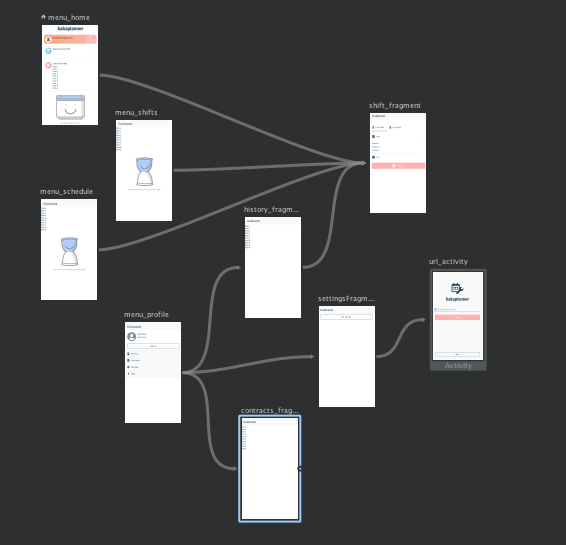
\includegraphics[scale=.65]{img/navigation.png}
% 	\caption{Hlavní navigační diagram}
% 	\label{fig:main-navigation}
% \end{figure}
%
% \subsubsection{Room}
% Room je knihovna pro perzistenci dat, která je abstraktní nadstavbou nad SQLite (relační databáze, kterou Android používá pro ukládání dat). Třídy dat jsou reprezenotvány jako entity (třídy značené \texttt{@Entity}). S~daty se interaguje skrz DAO\footnote{Data Access Object} (třída s~anotací \texttt{@Dao}), v němž se definují s~pomocí anotací (\texttt{@Query}, \texttt{@Insert}, \texttt{@Delete}, \texttt{@Update}) operace nad databází, SQL kód generuje knihovna. \cite{android2020room}
%
%
% \subsubsection{Data Binding}
% Data Binding Library\cite{android2020data} je knihovna, která umožňuje propojení UI komponent definovaných v~XML~layoutech s~daty. Pokud se celý layout obalí ve značce \texttt{<layout>\ldots</layout>}, vygeneruje knihovna kód (třídu implementující ab\-strakt\-ní \texttt{ViewDataBinding}), který zajistí propojení dat a layoutu; lze tak přímo v~layoutu definovat proměnné (zde lze definovat i ViewModel). Výhodou zde je i~snadné propojení LiveData a layoutu -- nastaví-li se pro binding \texttt{lifecycleOwner}, bude se o aktualizaci UI dle stavu LiveData starat knihovna.
%
% \begin{lstlisting}[language=XML]
% <TextView
% 	android:text="@{vm.user.firstName}"	/>
% \end{lstlisting}
%
% \subsubsection{Security}
%
% Security je knihovna pro zabezpečení souborů a SharedPreferences (úložiště pro primitivní páry klíč-hodnota, které se používá především na ukládání údajů o~uživateli). Keysety pro šifrování a dešifrování klíčů a hodnot se ukládají do SharedPreferences, a to v šifrované podobě (hlavní klíč pro šifrování a dešifrování keysetů je uložen v~Android Keystore, systémovém úložisti pro kryptografické klíče). \cite{android2021security}

% \section{Nástroje pro implementaci}
% Zde budou představeny nástroje a knihovny, které aplikaci nepřidávají funkcionalitu a od kterých by měl být uživatel odstíněn, ale byly použity při implementaci (aby usnadnily vývoj či hledání chyb).

% \subsubsection{Android Studio}
% Android Studio je oficiální IDE\footnote{Integrated development environment}, které v~sobě zahrnuje sadu nástrojů pro vývoj, testování, build a analýzu aplikací pro platformu Android.
%
% \subsubsection{Firebase Crashlytics}
% Firebase Crashlytics\footnote{\url{https://firebase.google.com/products/crashlytics}} je součást platformy Firebase, která poskytuje analýzu pádů aplikace včetně stack trace (viz obr. \ref{fig:crashlytics}) a údajů o zařízení, na němž k~chybě došlo (viz obr. \ref{fig:crashlytics-device}).
%
% \begin{figure}[h!]
% 	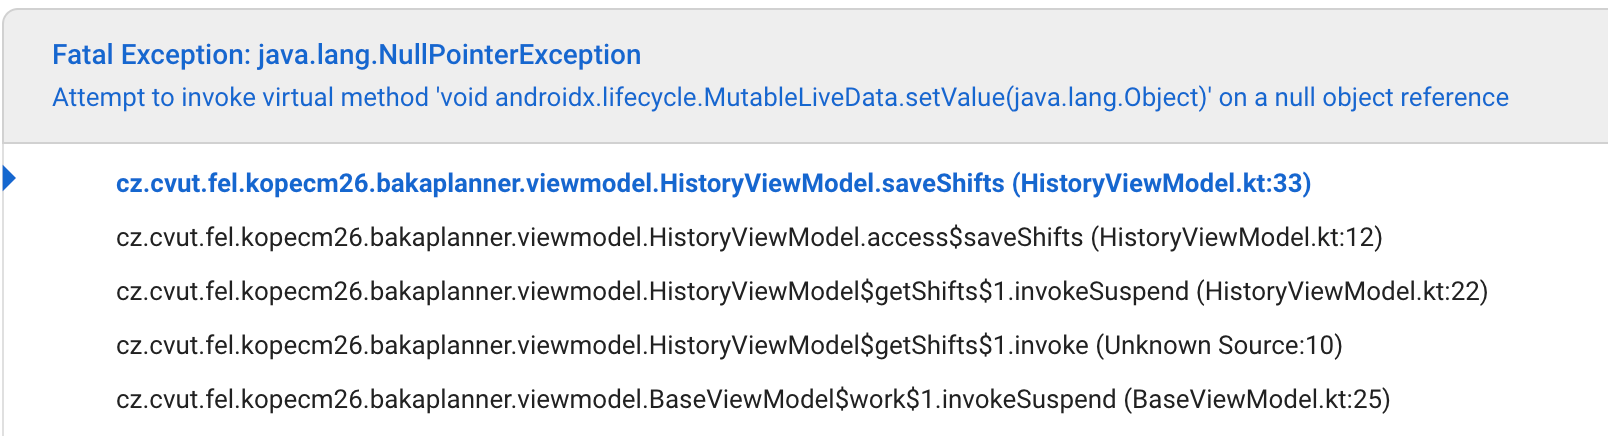
\includegraphics[scale=.45]{img/crashlytics.png}
% 	\caption{Ukázka stack trace v~Crashlytics}
% 	\label{fig:crashlytics}
% \end{figure}
%
% \begin{figure}[h!]
% 	
\includegraphics[scale=.45]{img/crashlytics_device.png}
% 	\caption{Ukázka údajů o~zařízení v~Crashlytics}
% 	\label{fig:crashlytics-device}
% \end{figure}
%
% \subsubsection{Lynx}
% Knihovna Lynx umožňuje zobrazit logy aplikace přímo v~mobilním telefonu, logy lze zobrazit jak v~samostatné aktivitě (např. po stisku tlačítka nebo po zatřesení telefonem), tak v~libovolném layoutu. \cite{sanchez2020lynx}

% \begin{figure}[ht]
% 	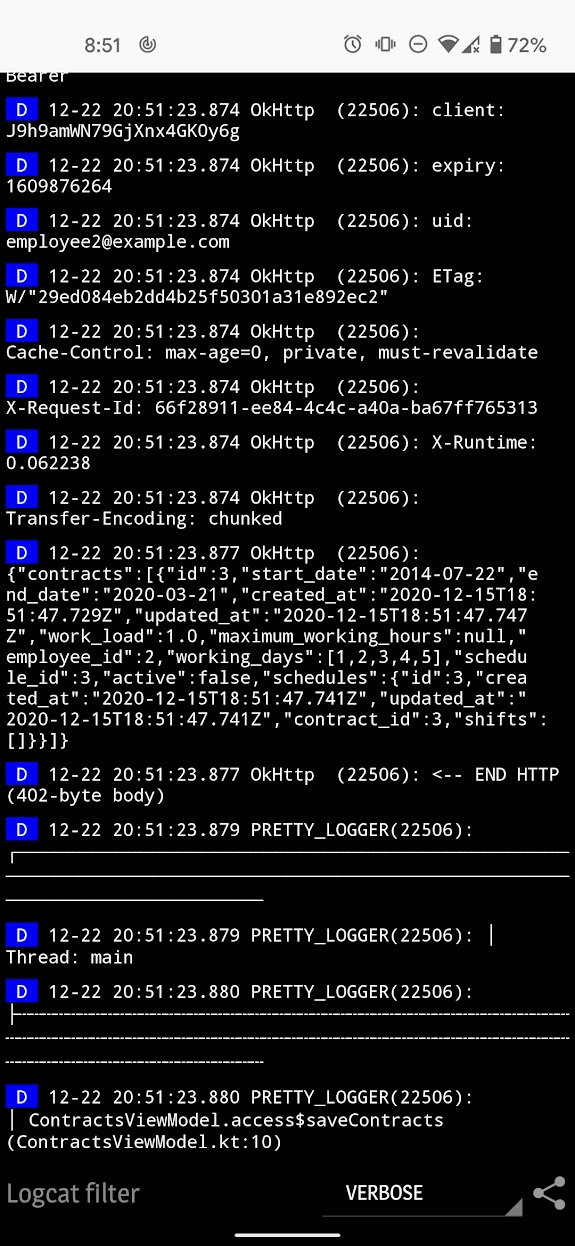
\includegraphics[scale=.3]{img/lynx.jpg}
% 	\caption{Logy v LynxActivity}
% 	\label{fig:lynx}
% \end{figure}

% \subsubsection{Logger}
% Logger \cite{obut2020logger} je jednoduchá knihovna pro logování, která vyžaduje minimum konfigurace.

\newpage
\section{Architektura aplikace}

Mobilní aplikace byla navrhnuta dle zásad nejpoužívanější a ze stranu Googlu doporučované architektury MVVM (vzhledem k~před\-po\-klá\-da\-né nízké komplexnosti aplikace zde nebyla implementována Clean Architecture, která vyžaduje vytvoření velkého množství komunikujících modulů).

Při implementaci byly využity především knihovny Koin (pro dependency injection), Retrofit (HTTP klient) a dále některé součásti Android Jetpack (soubor knihoven pro platformu Android, které usnadňují vývoj udržitelných aplikací a poskytují kompatibilitu se staršími verzemi OS \cite{android2020jetpack}), a to především LiveData (pozorovatelná data respektující životní cyklus Android UI komponent), Navigation (navigace mezi fragmenty aplikace), DataBinding (propojení UI komponent definovaných v~XML~layoutech s~daty) nebo Room (nadstavba nad databázi SQLite pro perzistenci dat).

Jedná se o~aplikaci s~nižším počtem aktivit (samostatné aktivity se využívají v~případě, že by nebylo vhodné zobrazovat v~aplikaci spodní navigaci, což znamená tehdy, když se vytváří nové zdroje, např.~nový zaměstnanec), v~níž navigace probíhá s~pomocí komponenty Navigation (např. detaily směn tedy nejsou sa\-mos\-tat\-ný\-mi aktivitami, ale jedná se o~fragmenty v~aktivitě \texttt{MainActivity}). Tento přístup k~navigaci byl odpozorován např.~u aplikací Spotify, YouTube nebo Instagram.

\subsection{View}

Pro zjednodušení vytváření nových aktivit při implemetaci byla vytvořena abstraktní třída \texttt{BindingActivity<B: ViewDataBinding>}, jež přijímá v~kon\-struk\-to\-ru jako parametr layout, každá konkrétní implementace této třídy ho tedy musí definovat (měl by být základem pro vygenerovanou třídu \texttt{B}). Abstraktní aktivita nastaví layout a binding, který je pro potomky přístupný jako proměnná \texttt{binding}, a~nastaví mu vlastníka životního cyklu.

Třída \texttt{ViewModelActivity<V: BaseViewModel, B:  ViewDataBinding>} je abstraktnim potomkem \texttt{BindingActivity}, který je přípraven pro aktivity, které mají vazbu na ViewModel (parametry konstruktoru jsou layout a třída ViewModelu). Tato aktivita zajišťuje vytvoření ViewModelu (který se uloží do proměnné \texttt{viewModel} a navíc se nastaví jako parametr pro binding).

Velmi podobně jako \texttt{BindingActivity} a \texttt{ViewModelActivity} fungují také abstraktní fragmenty, tj. \texttt{BindingFragment} a \texttt{ViewModelFragment}.

Vzhledem k~použití knihovny LiveData (pozorovatelná data závislá na životním cyklu aktivity/fragmentu) zde větší míře použit návrhový vzor Observer, View tedy pozoruje změny ViewModelu a podle toho se mění data.

\subsection{ViewModel}

ViewModely jsou v~této aplikaci potomkem abstraktní třídy \texttt{BaseViewModel}, která v~sobě obsahuje odkazy na všechny repositáře (inicializace je tzv. \textit{lazy}); také obsahuje LiveData pro zobrazování chyb a metody pro zpracování chyb a dat (to vše proto, aby se méně opakoval stejný kód). ViewModel ukládá odpovědi z~repozitářů jako LiveData (obecně by repozitáře měly být odstíněny od specifik platformy).

\subsection{Model}

Vrstva je v~této aplikaci realizována jako repozitáře. Ty mají zodpovědnost za provolání správných datových zdrojů, jimiž jsou lokální databáze a vzdálený zdroj (tzn.~provolání cesty na serveru), a za ukládání dat do databáze či do cache. Odpovědi se vracejí obalené ve třídě \texttt{ResponseModel<T>} (viz kód~\ref{lst:responsemodel}), která může nést zprávu o chybě nebo požadovaná data. O~dalším osudu této odpovědi rozhoduje ViewModel.

\begin{lstlisting}[language=Kotlin,caption={Třída \texttt{ResponseModel}},label={lst:responsemodel}]
sealed class ResponseModel<T> {
	class SUCCESS<T>(var data: T? = null, val headers: Headers? = null): ResponseModel<T>()

	class ERROR<T>(val errorType: ErrorType? = null): ResponseModel<T>()
}
\end{lstlisting}

\section{Design}\label{design}

Design aplikace vznikl v souladu se základními pravidly Material Designu. Jako inspirace zde sloužil především minimalismus aktuálních veřejně dos\-tup\-ných aplikací, jako jsou například Instagram, Google Fit nebo Spotify. Základní návrh prvků uživatelského rozhraní byl načrtnut v~nástroji Figma (konkrétní podoba obrazovek však vznikala až při implementaci). Ikonky byly převzaty z~knihoven Font Awesome 5 (fas) a Material Design Icon (mdi), ilustrace byly vytvořeny v~programu Sketch. Pro konkrétní návrhy viz~přílohu \todo{Příloha design}

% \chapter{Stav implementace}
%
% Aplikace byla prozatím testována pouze v~lokální síti a pouze na náhodně vygenerovaných testovacích datech. Testovací data se na straně serveru generují seedují\footnote{Seedování je proces, kterým se inicializují počáteční data v~databázi.}, nadefinovány jsou seedy pro uživatelské účty (vygenerují se účty employee1 až employee10, každý s~heslem \uv{12345678}). Uživatelům jsou náhodně vytvořeny a přiřazeny smlouvy a směny.
%
% Během implementace aplikace byl důraz kladen především na uživatelské rozhraní aplikace pro zaměstnance. Byla tak implementována ta část obrazovek, kterou potřebují aktuálně definované případy užití této aplikace a patřičné části backendu.
%
% \section{Implementace případů užití}
%
% V~této části bude rozebrána konkrétní implementace případů užití popsaných v~podkapitole~\ref{uc-analysis}. Součástí jsou i~snímky obrazovky z~mobilní aplikace.
% \newpage
%
% \subsection{UC1: Přihlásit se}
% Pro tento případ užití je připravena aktivita \texttt{SetupActivity}. Vzhledem k~tomu, že tato aplikace momentálně běží v~lokální síti a adresa backendu se může měnit, začíná scénář obrazovkou \uv{Zadejte URL backendu} (viz obr.~\ref{fig:uc1-url}). Po stisknutí tlačítka \uv{Nastavit} proběhne validace textového formuláře s~pomocí knihovny VValidator a je-li zadána validní URL, uloží se adresa backendu do SharedPreferences a~změní se fragment v~aktivitě na přihlašovací formulář (viz obr.~\ref{fig:uc1-login}), zde opět po stisknutí tlačítka \uv{Přihlásit se} proběhne validace formuláře, zda je vyplněn.
%
% \begin{figure}[h]
% 	\centering
% 	\begin{subfigure}{.5\textwidth}
% 		\centering
% 		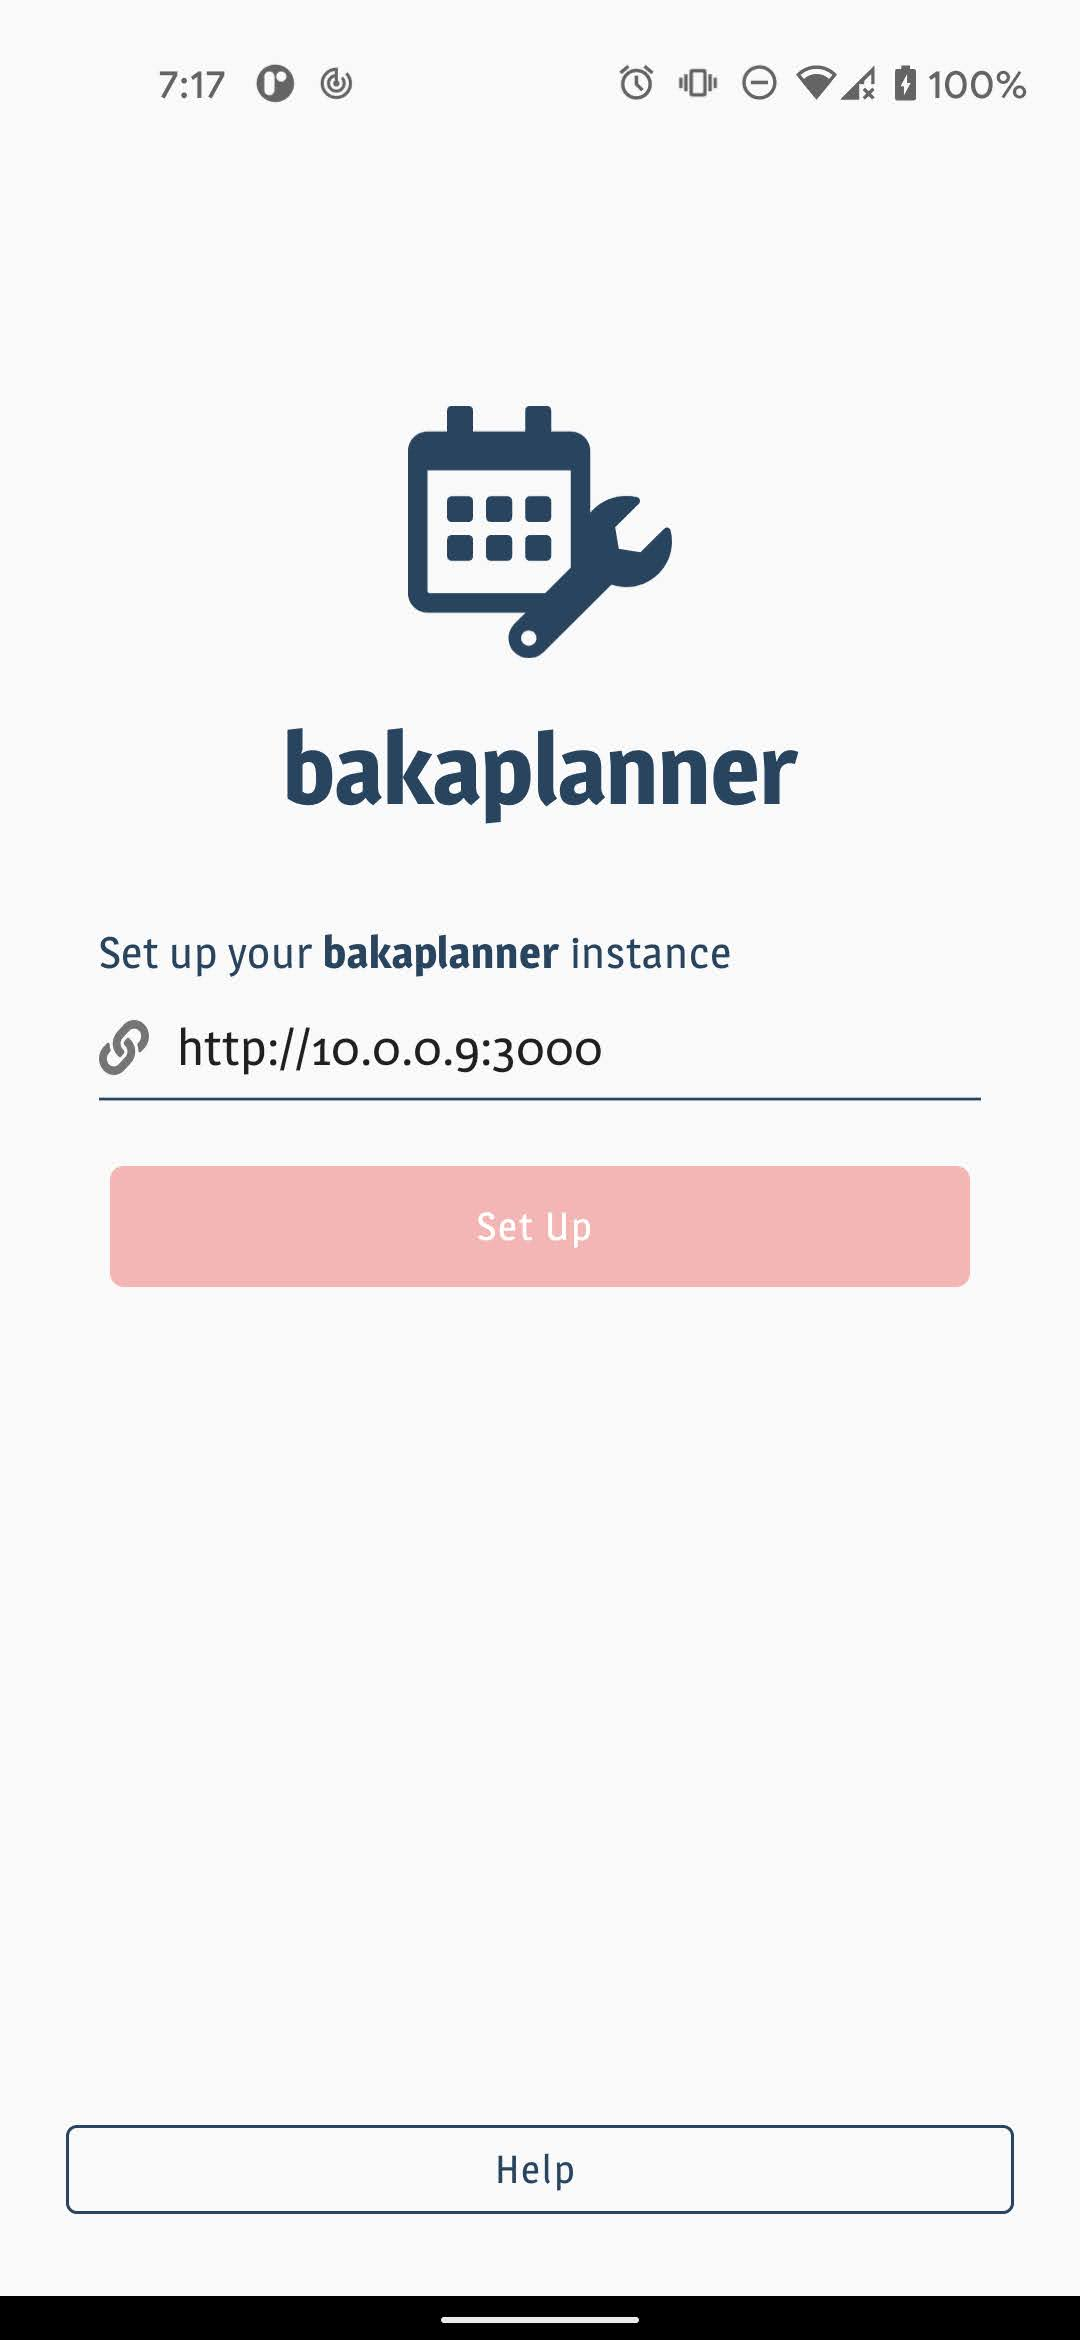
\includegraphics[width=.9\linewidth]{img/uc1_screen001.jpg}
% 		\subcaption{Zadejte URL backendu}
% 		\label{fig:uc1-url}
% 	\end{subfigure}%
% 	\begin{subfigure}[h!]{.5\textwidth}
% 		\centering
% 		
\includegraphics[width=.9\linewidth]{img/uc1_screen002.jpg}
% 		\subcaption{Zadejte přihlašovací údaje}
% 		\label{fig:uc1-login}
% 	\end{subfigure}
% 	\caption{Obrazovky pro scénář UC1: Přihlásit se}
% \end{figure}
%
% Jsou-li údaje všechny údaje vyplněny, odešle se požadavek (\texttt{POST} na endpoint \texttt{/auth/sign\_in} s~u\-ži\-va\-tel\-ským jménem a heslem v~těle požadavku) na server. Na serveru se požadavek zpracuje, o což se stará knihovna Devise Token Auth. Server může vrátit stavové kódy dle podkapitoly \ref{sub:sign-in}. V~případě neúspěchu je zobrazen Snackbar\footnote{Snackbar je UI komponenta pro zobrazování krátkých zpráv o~stavu aplikace, jedná se o~součást Material Design Library.} s popisem chyby; naopak pokud je požadavek úspěšný, server vrátí údaje o uživateli a přístupové tokeny (viz podkapitolu \ref{sub:devise}), které se na straně klienta uloží do SharedPreferences, aby se mohy posílat s~každým dalším požadavkem. Tím je tento scénář ukončen a uživatel je navigován do \texttt{MainActivity}.
%
%
%
% \subsection{UC2: Odhlásit se}
%
% Pokud je uživatel na obrazovce Profil (obr.~\ref{fig:uc2-profile}, tzn.~\texttt{ProfileFragment}), je jedinou věcí, co musí uživatel udělat, aby se odhlásil, stisknutí tlačítka Odhlásit se. Tím se odešle na server požadavek \texttt{DELETE /auth/sign\_out} s~hlavičkami s~tokenem, které jsou uloženy v SharedPreferences. Pokud je odpověď ze serveru 200 -- OK nebo 404 -- Not Found (to znamená, že token nebyl nalezen; každopádně by toto mělo zaručit, že uživatel bude z~aplikace odhlášen, i když se změní data na serveru), odstraní se všechny údaje o~uživateli a~všechna data uložená v~databázi. Uživatel je vrácen na obrazovku Přihlášení, tím je scénář ukončen.
%
% \begin{figure}[ht]
% 	
\includegraphics[width=.45\linewidth]{img/uc2-profile.png}
% 	\caption{Obrazovka Profil}
% 	\label{fig:uc2-profile}
% \end{figure}
%
% \subsection{UC3: Zobrazit rozvrh směn}
% \label{sub:uc3}
%
% Rozvrh směn se zobrazuje na stránce Rozvrh (fragment \texttt{ScheduleFragment}). Pokud nejsou žádné směny uloženy v~databázi, odešle se \texttt{GET} požadavek na \texttt{/shifts} (o tom, zda se požadavek odešle, rozhoduje \texttt{ShiftRepository}). V~případě, že po odeslání požadavku na server dojde k~nějaké chybě, zobrazí se Snackbar s~popisem chyby. Pokud v~repozitáři nedojde k~chybě, udělá se dotaz na lokální databázi a vrátí se patřičné směny, které se zobrazí v~seznamu (obr.~\ref{fig:uc2-schedule-app}); pokud je seznam směn prázdný, zobrazí patřičnou hlášku (obr.~\ref{fig:uc2-schedule-app-empty}). Tato obrazovka (stejně jako zbytek seznamů) implementuje swipe to refresh -- uživatel tedy gestem \uv{swipe} může vynutit odeslání požadavku na server.
%
% \begin{figure}[ht]
% 	\centering
% 	\begin{subfigure}{.5\textwidth}
% 		\centering
% 		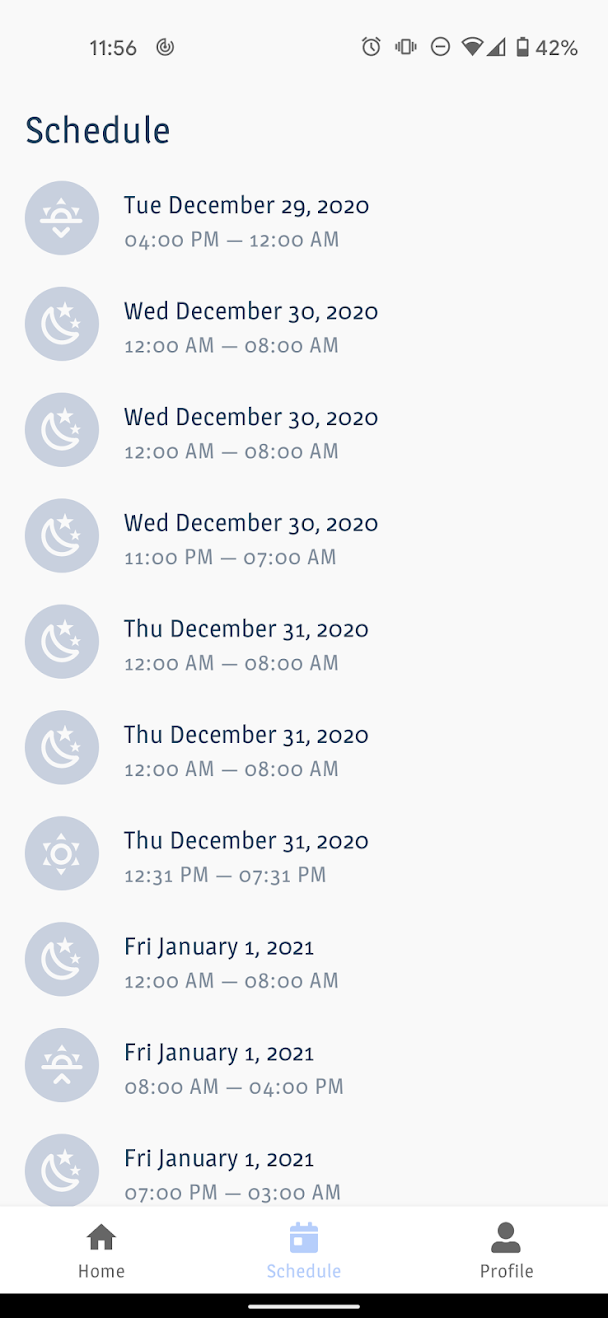
\includegraphics[width=.9\linewidth]{img/uc3-schedule.png}
% 		\subcaption{Seznam směn}
% 		\label{fig:uc2-schedule-app}
% 	\end{subfigure}%
% 	\begin{subfigure}[h!]{.5\textwidth}
% 		\centering
% 		
\includegraphics[width=.9\linewidth]{img/uc3-schedule-empty.jpg}
% 		\subcaption{Seznam směn je prázdný}
% 		\label{fig:uc2-schedule-app-empty}
% 	\end{subfigure}
% 	\caption{Obrazovky pro scénář UC3: Zobrazit rozvrh směn}
% \end{figure}
%
% \subsection{UC4: Zobrazit detail směny}
%
% Detail směny se zobrazuje v~\texttt{ShiftFragment} (viz obr.~\ref{uc4}), který přijímá jako argument \texttt{Shift}. Všechna data jsou už dostupná v~seznamu směn, z~něhož se do detailu naviguje, \texttt{ShiftFragment} je pouze zobrazuje. Na této obrazovce se v~určitých případech může zobrazovat tlačítko Zapsat směnu nebo Zrušit zápis na směnu.
%
% \begin{figure}[ht]
% 	
\includegraphics[width=.45\linewidth]{img/uc4.jpg}
% 	\caption{Obrazovka Detail směny}
% 	\label{uc4}
% \end{figure}
% \newpage
%
% \subsection{UC5: Zobrazit přehled nejbližších směn}
%
% Přehled nejbližších směn se ukazuje na domovské obrazovce (tedy ve fragmentu \texttt{HomeFragment}, viz obr.~\ref{uc5}). \texttt{HomeViewModel} žádá repozitář o data -- pokud v~databázi nic není, odešle se \texttt{GET} požadavek na seznam následujích směn, tedy na endpoint \texttt{/shifts}. Relevantní data (aktuálně probíhající směna, následující směna, směny v~tomto kalendářním týdnu) se získají dotazem do lokální databáze.
%
% \begin{figure}[ht]
% 	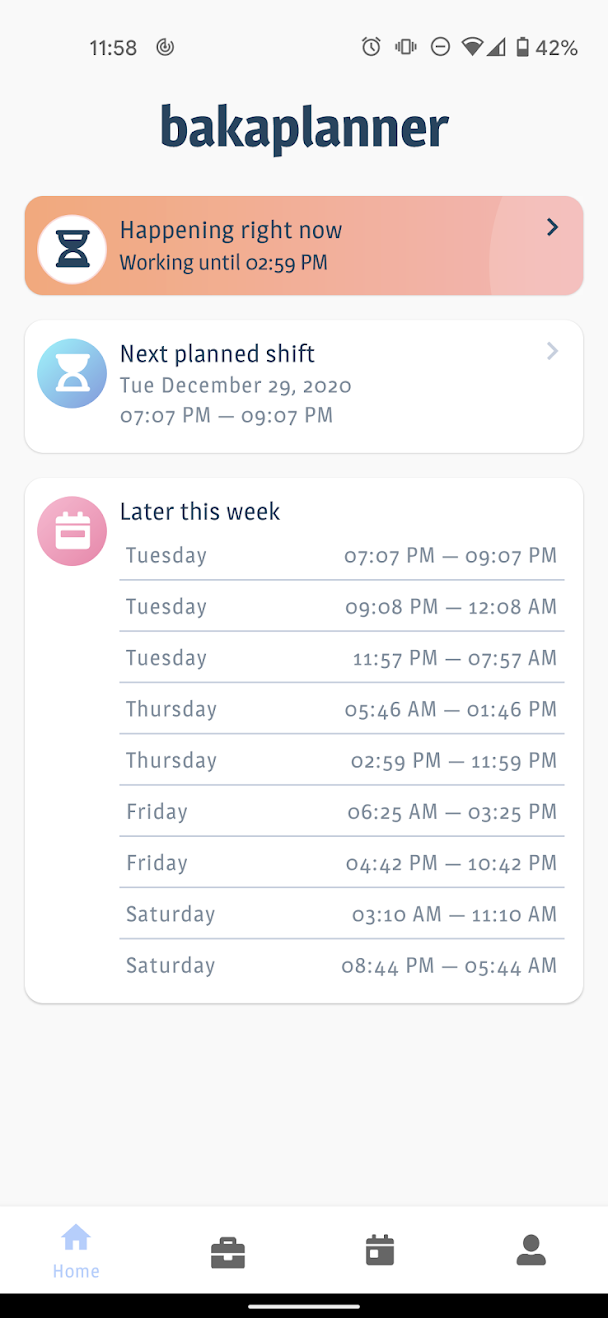
\includegraphics[width=.45\linewidth]{img/uc5.png}
% 	\caption{Domovská obrazovka s~přehledem nejbližších směn}
% 	\label{uc5}
% \end{figure}
% \newpage
%
%
% \subsection{UC6: Zobrazit historii odpracovaných směn}\label{sub:uc6}
%
% Pokud je uživatel na obrazovce Profil (obr.~\ref{fig:uc2-profile}), může otevřít obrazovku Historie (\texttt{HistoryFragment}, obr.~\ref{uc6}). Celý scénář je velmi podobný jako scénář pro Zobrazit rozvrh směn (viz podkapitolu \ref{sub:uc3}) nebo Zobrazit seznam, hlavním rozdílem je to, jaká data se vracejí (\texttt{end\_date} směny už uplynulo) a jak seřazená jsou (sestupně dle \texttt{start\_date}).
%
% \begin{figure}[ht]
% 	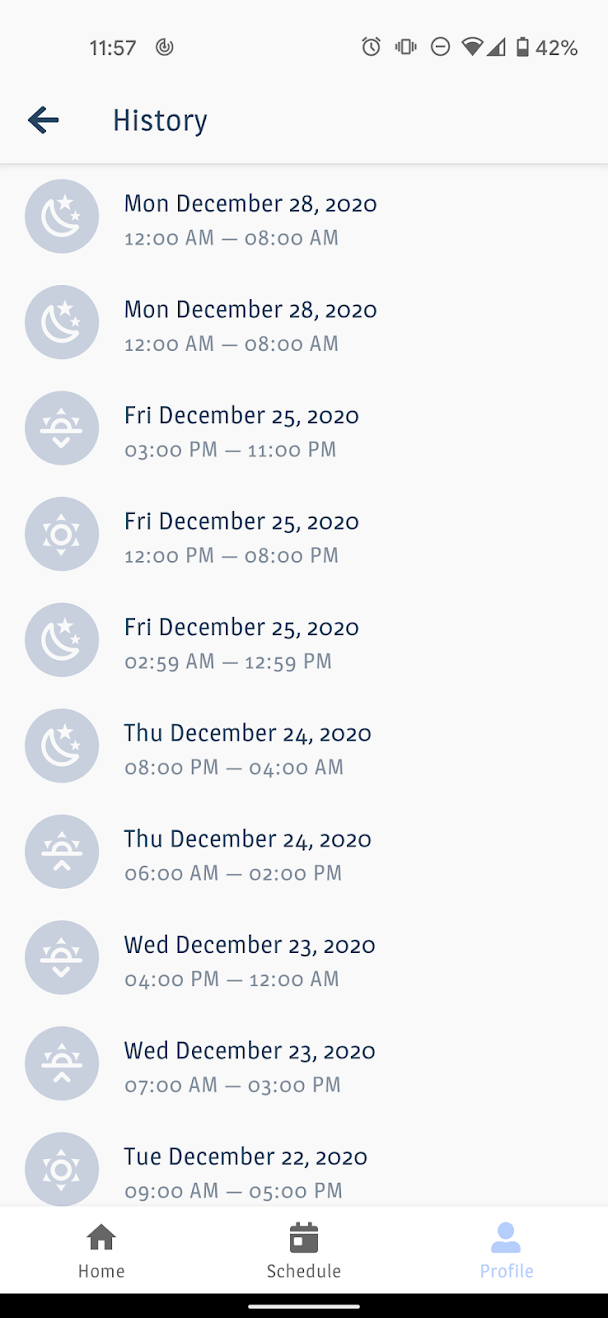
\includegraphics[width=.45\linewidth]{img/uc6.png}
% 	\caption{Obrazovka s~historií směn}
% 	\label{uc6}
% \end{figure}
% \newpage
%
% \subsection{UC7: Zobrazit přehled smluv}
%
% Pokud je uživatel na obrazovce Profil (obr.~\ref{fig:uc2-profile}), může otevřít obrazovku Smlouvy (viz~obr.~\ref{uc7}). Nejsou-li uloženy v~lokální databázi, posílá se \texttt{GET} požadavek na \texttt{/contracts}, je-li úspěšný, smlouvy se ukládají do lokální databáze. Smlouvy jsou rozděleny na aktuální a neaktuální, a to dle data začátku a konce.
%
% \begin{figure}[ht]
% 	
\includegraphics[width=.45\linewidth]{img/uc7.png}
% 	\caption{Přehled smluv}
% 	\label{uc7}
% \end{figure}
% \newpage
%
% \subsection{UC8: Zobrazit seznam volných směn}
%
% Jedná se o případ užití, který je velmi podobný jako Zobrazit seznam směn (viz~\ref{sub:uc3}) nebo Zobrazit historii odpracovaných směn \ref{sub:uc6}. Tentokrát uživatel musí otevřít záložku Volné směny (\texttt{UnassignedFragment}, obr.~\ref{uc8}); hlavním rozdílem je, že se volné směny neukládají do lokální databáze, neboť tato data by m+la být pokud možno vždy aktuální.
%
% \begin{figure}[ht]
% 	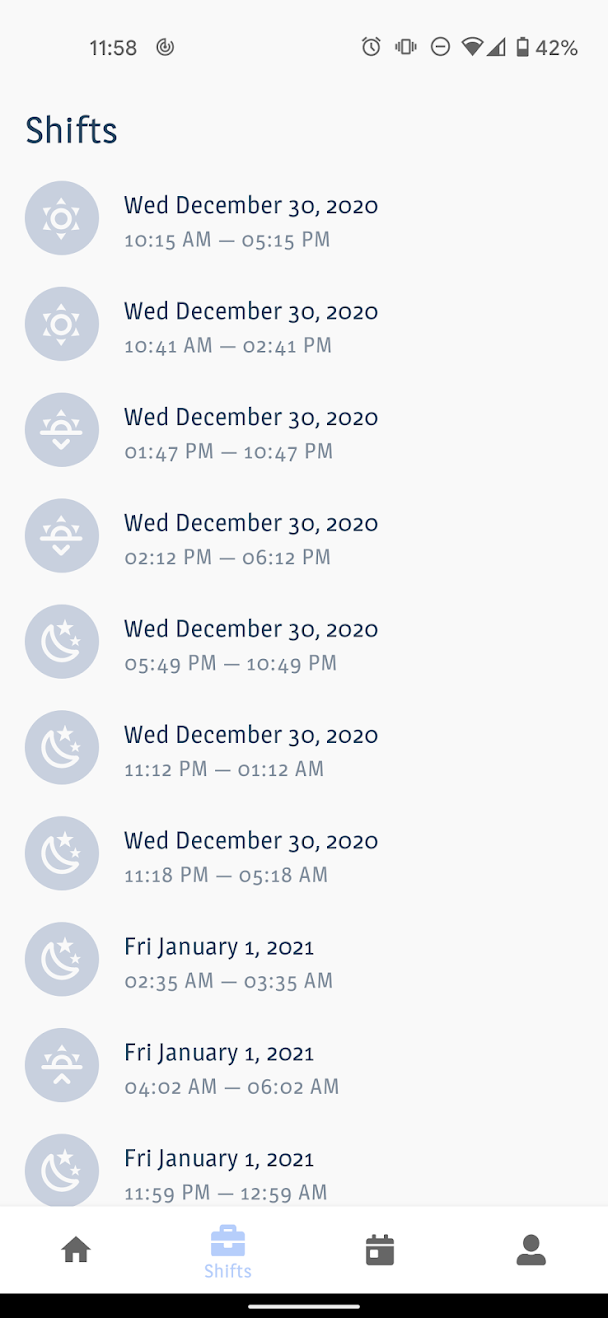
\includegraphics[width=.45\linewidth]{img/uc8.png}
% 	\caption{Přehled smluv}
% 	\label{uc8}
% \end{figure}
% \newpage
%
%
% \subsection{UC9: Zapsat se na volnou směnu}
%
% Na obrazovce Detail směny se může zobrazit tlačítko \uv{Zapsat se na směnu} (obr.~\ref{uc9a}), a to v~případě, že směna není zapsána do žádného rozvrhu. Pokud uživatel na toto tlačítko klikne, zobrazí se obrazovka Vybrat rozvrh, po jejíž inicializaci se odešle \texttt{GET} požadavek na seznam všech rozvrhů, do nichž lze směnu zapsat (na \texttt{/shift/:id/schedules}). Rozvrhy se zobrazí v~seznamu (je-li požadavek úspěšný), uživatel nějaký vybere a odešle se \texttt{POST} požadavek na \texttt{/shift/:id/schedule} s~id rozvrhu jako parametrem (toto má ten význam, bude-li zaměstnanec mít více smluv a~více rozvrhů). V~případě úspěchu se ze serveru vrátí směna, která se uloží do~lokální databáze. Uživatel je vrácen na obrazovku Volné směny, zobrazí se Snackbar se zprávou o úspěchu a~znovu se načtou data ze serveru.
%
% \begin{figure}[ht]
% 	\centering
% 	\begin{subfigure}{.5\textwidth}
% 		\centering
% 		
\includegraphics[width=.9\linewidth]{img/uc9a.png}
% 		\subcaption{Detail směny}
% 		\label{uc9a}
% 	\end{subfigure}%
% 	\begin{subfigure}[h!]{.5\textwidth}
% 		\centering
% 		
\includegraphics[width=.9\linewidth]{img/uc9b.png}
% 		\subcaption{Vyberte rozvrh}
% 		\label{uc9b}
% 	\end{subfigure}
% 	\caption{Obrazovky pro scénář UC9: Zapsat se na volnou směnu}
% \end{figure}
%
% \subsection{UC10: Zrušit zápis na směnu}
%
% Zápis na směnu lze zrušit na obrazovce Detail směny (obr.~\ref{uc10a}), a to v~tom případě, že byla směna naplánována uživatelem a začíná za méně než 4 dny (v~opačném případě se tlačítko \uv{Zrušit zápis na směnu} vůbec nezobrazí). Pokud uživatel klikne na dané tlačítko, zobrazí se dialog Jste si jisti? (obr.~\ref{uc10b}). Pokud uživatel klikne jinam než na tlačítko Ano, dialog zmizí a nic se nestane; pokud smazání potvrdí, pošle se \texttt{DELETE} požadavek na \texttt{/shifts/:id/schedule}. V~případě úspěchu se ze serveru vrátí tato směna, která se následně smaže z~lokální databáze. Uživatel je vrácen na obrazovku Rozvrh směn, zobrazí se Snackbar se zprávou o úspěchu a~znovu se načtou data z~databáze.
%
% \begin{figure}[ht]
% 	\centering
% 	\begin{subfigure}{.5\textwidth}
% 		\centering
% 		
\includegraphics[width=.9\linewidth]{img/uc10a.png}
% 		\subcaption{Detail směny s~tlačítkem Odstranit z~rozvrhu}
% 		\label{uc10a}
% 	\end{subfigure}%
% 	\begin{subfigure}[h!]{.5\textwidth}
% 		\centering
% 		
\includegraphics[width=.9\linewidth]{img/uc9b.png}
% 		\subcaption{Dialog Jste si jisti?}
% 		\label{uc10b}
% 	\end{subfigure}
% 	\caption{Obrazovky pro scénář UC10: zrušit zápis na směnu}
% \end{figure}

\chapter{Závěr}

% V~rámci tohoto semestrálního projektu byla provedena analýza problematiky rozvrhování směn, a to jak manažerského, tak z~hlediska legislativy v~oblasti rozvrhování směn, na jejímž základě byly sestaveny funkční požadavky na mobilní aplikaci pro plánování lidských zdrojů.
%
% V~části implementace aktuálně je připraveno mobilní rozhraní pro za\-měst\-nan\-ce, které dostává testovací data ze serveru.
%
% Tento projekt bude dále pokračovat jako bakalářská práce, plánem je dále zlepšovat uživatelské rozhraní aplikace pro zaměstnance, jakož i vytvářet nové funkcionality a nové případy užití (např. rozhraní pro vedoucího pracovníka), zároveň bude třeba implementovat na základě analýzy algoritmů automatické sestavování rozvrhů. Zároveň je výhledem, bude-li to možné, i~testování aplikace na několika uživatelích.

\printbibliography[title={Seznam použité literatury}]

\appendix

% \chapter{Seznam použitých zkratek}
% \glsaddall
% \printnoidxglossaries
%
% \chapter{Design mobilní aplikace}\label{app:design}



\chapter{Internetové odkazy}
\section{Uživatelské příběhy}\label{sec:user-story}

Mapa uživatelských příběhů v plné velikosti
\begin{itemize}
	\item \url{https://github.com/kopemar/baka-docs/blob/main/storyboard.pdf}
\end{itemize}


\section{Návrh uživatelského rozhraní}\label{sec:ui}

Wireframes, mapa obrazovek v mobilní aplikaci
\begin{itemize}
	\item \url{https://github.com/kopemar/baka-docs/blob/main/lfp.pdf}
\end{itemize}




% Zde je seznam ikonek, které byly použity v~aplikaci včetně jejich zdroje (fas značí knihovnu Font Awesome 5\footnote{\url{https://fontawesome.com/}}; mdi Material Design Icon\footnote{\url{https://material.io/resources/icons/}})
% \begin{figure}[h!]
% 	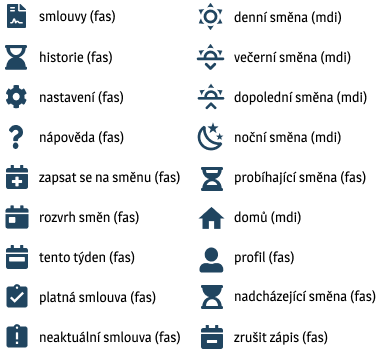
\includegraphics[scale=.7]{img/icons.png}
% 	\caption{Použité ikonky}
% 	\label{fig:icons}
% \end{figure}
% \newpage
% \section{Logo aplikace}
%
% V~logu aplikace byly použity ikonky z~knihovny Font Awesome 5.
%
% \begin{figure}[h!]
% 	
\includegraphics[scale=.5]{img/logo.png}
% 	\caption{Logo aplikace}
% 	\label{fig:logo}
% \end{figure}
%
% \begin{figure}[h]
% 	\centering
% 	\begin{subfigure}{.5\textwidth}
% 		\centering
% 		
\includegraphics[width=.7\linewidth]{img/launcher-prod.png}
% 		\subcaption{Verze Release}
% 		\label{launcher-prod}
% 	\end{subfigure}%
% 	\begin{subfigure}[h!]{.5\textwidth}
% 		\centering
% 		
\includegraphics[width=.7\linewidth]{img/launcher-debug.png}
% 		\subcaption{Verze Debug}
% 		\label{launcher-debug}
% 	\end{subfigure}
% 	\caption{Ikona Android aplikace}
% \end{figure}
%
% \section{Ilustrace}\label{ilu}
% \begin{figure}[h]
% 	\centering
% 	\begin{subfigure}[b]{.24\textwidth}
% 		\centering
% 		
\includegraphics[width=.6\linewidth]{img/il-upcoming.png}
% 		\subcaption{Budoucí směny}
% 		\label{fig:il-upcoming}
% 	\end{subfigure}%
% 	\begin{subfigure}[b]{.24\textwidth}
% 		\centering
% 		
\includegraphics[width=.6\linewidth]{img/il-history.png}
% 		\subcaption{Historie směn}
% 		\label{fig:il-history}
% 	\end{subfigure}
% 	\begin{subfigure}[b]{.24\textwidth}
% 		\centering
% 		
\includegraphics[width=.9\linewidth]{img/il-schedule.png}
% 		\subcaption{Rozvrh směn}
% 		\label{fig:il-schedule}
% 	\end{subfigure}%
% 	\begin{subfigure}[b]{.24\textwidth}
% 		\centering
% 		
\includegraphics[width=.9\linewidth]{img/il-connection.png}
% 		\subcaption{Bez připojení}
% 		\label{fig:il-connection}
% 	\end{subfigure}
% 	\caption{Návrh ilustrací}
% \end{figure}
%
% \newpage
% \section{Návrh obrazovek}
% \begin{figure}[h]
% 	\centering
% 	\begin{subfigure}{.5\textwidth}
% 		\centering
% 		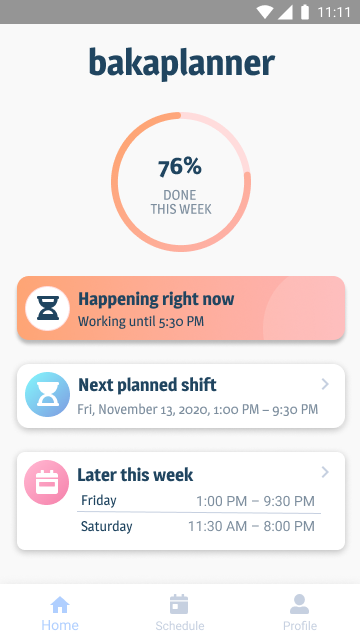
\includegraphics[width=.9\linewidth]{img/v1-main-home.png}
% 		\subcaption{Světlý režim}
% 		\label{fig:main-home}
% 	\end{subfigure}%
% 	\begin{subfigure}[h!]{.5\textwidth}
% 		\centering
% 		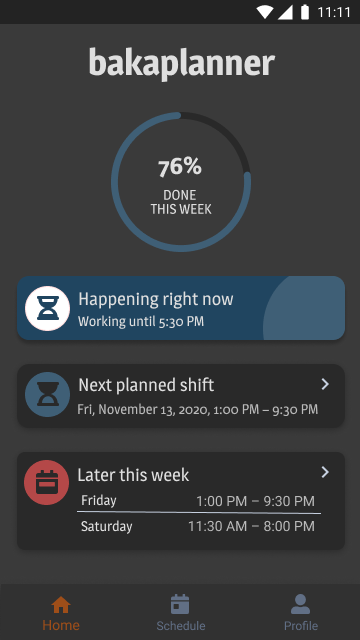
\includegraphics[width=.9\linewidth]{img/v1-main-home-night.png}
% 		\subcaption{Tmavý režim}
% 		\label{fig:main-home-dark}
% 	\end{subfigure}
% 	\caption{Návrh domovské obrazovky}
% \end{figure}
%
% \begin{figure}[h]
% 	\centering
% 	\begin{subfigure}{.5\textwidth}
% 		\centering
% 		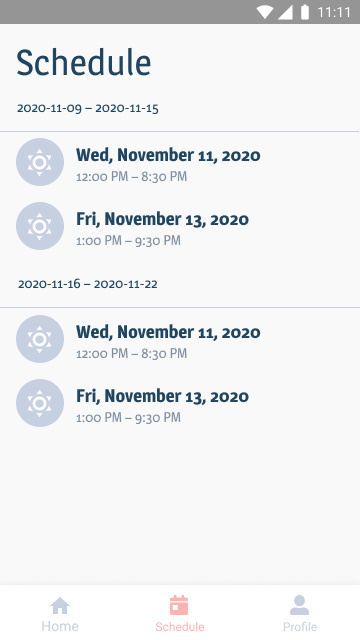
\includegraphics[width=.9\linewidth]{img/v1-main-home-schedule.png}
% 		\subcaption{Světlý režim}
% 		\label{fig:main-schedule}
% 	\end{subfigure}%
% 	\begin{subfigure}[h!]{.5\textwidth}
% 		\centering
% 		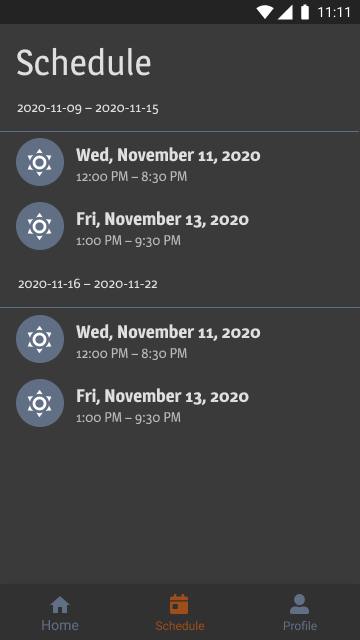
\includegraphics[width=.9\linewidth]{img/v1-main-home-schedule-night.png}
% 		\subcaption{Tmavý režim}
% 		\label{fig:main-schedule-dark}
% 	\end{subfigure}
% 	\caption{Návrh obrazovky rozvrh směn}
% \end{figure}
%
% \begin{figure}[h]
% 	\centering
% 	\begin{subfigure}{.5\textwidth}
% 		\centering
% 		
\includegraphics[width=.9\linewidth]{img/v1-main-home-schedule-empty.png}
% 		\subcaption{Světlý režim}
% 		\label{fig:main-schedule-empty}
% 	\end{subfigure}%
% 	\begin{subfigure}[h!]{.5\textwidth}
% 		\centering
% 		
\includegraphics[width=.9\linewidth]{img/v1-main-home-schedule-empty-night.png}
% 		\subcaption{Tmavý režim}
% 		\label{fig:main-schedule-dark-empty}
% 	\end{subfigure}
% 	\caption{Návrh obrazovky rozvrh směn (prázdný)}
% \end{figure}
%
% \begin{figure}[h]
% 	\centering
% 	\begin{subfigure}{.5\textwidth}
% 		\centering
% 		
\includegraphics[width=.9\linewidth]{img/v1-shift-detail.png}
% 		\subcaption{Bez tlačítka}
% 		\label{fig:v1-shift}
% 	\end{subfigure}%
% 	\begin{subfigure}[h!]{.5\textwidth}
% 		\centering
% 		
\includegraphics[width=.9\linewidth]{img/v1-shift-detail-button.png}
% 		\subcaption{S~tlačítkem}
% 		\label{fig:v1-shift-button}
% 	\end{subfigure}
% 	\caption{Návrh obrzovky detail směny}
% \end{figure}
%
% \begin{figure}[h]
% 	\centering
% 	\begin{subfigure}{.5\textwidth}
% 		\centering
% 		
\includegraphics[width=.9\linewidth]{img/v1-main-profile.png}
% 		\subcaption{Obrazovka Profil}
% 		\label{fig:v1-shift}
% 	\end{subfigure}%
% 	\begin{subfigure}[h!]{.5\textwidth}
% 		\centering
% 		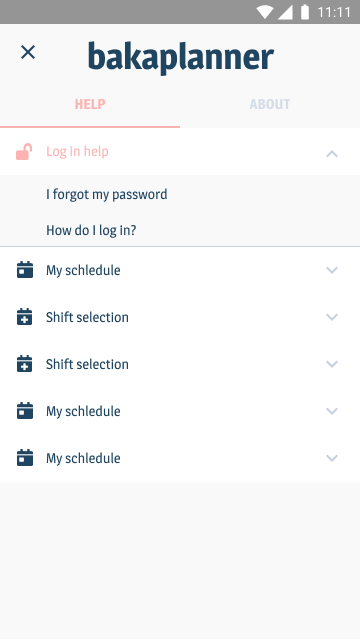
\includegraphics[width=.9\linewidth]{img/v1-help_interface.png}
% 		\subcaption{Obrazovka Nápověda}
% 		\label{fig:v1-shift-button}
% 	\end{subfigure}
% 	\caption{Návrh obrazovek Profil a Nápověda}
% \end{figure}

\newpage

\end{document}
